\chapter{EPR Spectroscopy of TEMPO--Salen Electrochemical Cells}
\label{ch:SPINS_AT_WORK}
Here the cwEPR spectra of TEMPO-Salen electrochemical cells are shown under operating conditions and ex situ, for various states of charge, as well as the spectra of the materials that were used to construct the cells.
That information is used to decompose the complex spectra of a charging cell and to perform its quantitative analysis to identify the state of charge of the cell and the by-products that are being released during the cell operation. The EPR-detected state of charge (ESOC), as inferred from the number of paramagnetic centres in the film, is compared to the results of Coulomb counting based on galvanostatic charging. Quantitative studies of cell degradation upon repeated charge-discharge cycling revealed the formation and growth of electrochemically inactive charge-storing domains in a cathode film. Quantitative measurements of a charged cell under open-circuit conditions allowed for connecting the self-discharge of the cell to the concentration of released redox active nitroxide fragments that serve as charge shuttles between the cathode and the anode. Low-temperature cwEPR spectra of TEMPO-salens at various SoC have shown the coexistence of domains with low and high spin concentration within the redox active film.


\section{cwEPR Spectroscopy of Working\\TEMPO-Salen Electrochemical Cells}
There is a number of difficulties when it comes to an EPR experiment on a working electrochemical cell. The cell must contain mobile ions between its electrodes - cations and anions. The ions are normally produced as products of dissociating salts. To overcome the ionic bond in a salt and to break it into the ions, a solvent with a large dipole moment is needed. Solvents with large dipole moments, such as acetonitrile (CH\textsubscript{3}CN, $\varepsilon\approx 37.5$) or water ($\varepsilon\approx78.4$), have large dielectric constants ($\varepsilon$) which results in a non-resonant absorption of microwaves~\footnote{The rotational energy levels of small polar molecules spread over the microwave domain~\cite{Dermtroeder}. The electrical component of the microwaves couples to the electric dipole moment of the molecule and increases its energy by exciting the rotational degrees of freedom. While this property is fundamental for microwave heating, in the EPR experiments it is undesired. Therefore, in an EPR experiment, one separates the electric and magnetic components of the microwave in a resonator. For an EPR experiment on a working battery, the liquid electrolytes and metals change the distribution of the electric field in the resonator, so measures have to be taken to avoid the heating of the sample.}. A cell containing liquid electrolyte absorbs microwaves and lowers the sensitivity of the EPR experiment. Furthermore, due to a finite dimension of cell, not only the magnetic component of the microwave is interacting with the electrolyte, but also the electric one - this results in heating of the electrolyte in a similar fashion as in a microwave oven. The heating of the electrolyte leads to a faster degradation of the cell and does not allow for long systematic measurements.\\
Another general issue with the operando EPR and EDMR experiments is that the device under testing (DUT) has to have metal electrodes that deliver current to it. Metals, placed in a microwave cavity, change the distribution of the electromagnetic field in it - that weakens the magnetic component at the device and at the same time strengthens the electric component. It is the magnetic dipole transition that is causing the magnetic resonance, so the weakening of the magnetic component by introducing the metal electrodes further decreases the magnetic resonance response. The increased electric component causes heating to temperatures that can be critical for the DUT operation.

\subsection{Spectra of TEMPO--Containing Molecular Fragments}
% todo: the reader knows about TEMPO, dits and ditbus. Show how they behave in cwEPR spectrometer.
% picture of molecule - spectrum - diagram
The stable TEMPO$^\bullet$ radical is widely used in the EPR spectroscopy as a spin probe and particularly in the EPR studies of TEMPO containing ORB materials~\cite{nakahara2002_cpl, nishide2004_electact, bahaceci2013_jpowersources, aydin2015_jsoistatelect, khodeir2019_softmatter, Zhang2018}. The spin density at the TEMPO$^\bullet$ radical is localized within the N-O bond~\cite{Owenius2001} and partially resides on the $I=1$ $^{14}$N nucleus, so to describe the EPR spectrum of an isolated TEMPO$^\bullet$ one has to take into consideration the electron Zeeman term $H_{EZ}$, the nuclear Zeeman term $H_{NZ}$ and the hyperfine coupling term $H_{HF}$. The unpaired electron spin on TEMPO$^\bullet$ has anisotropic $g$ values, because of the asymmetry of its molecular orbital, so the $\textbf{g}$ matrix and the $\textbf{A}$ hyperfine coupling tensor are both anisotropic. $\textbf{g}$ is diagonal in the molecular frame of reference shown in Figure~\ref{fig:TEMPO_dft}. Its principal values are $\left[g_{xx}=2.009,g_{yy}=2.006,g_{zz}=2.002\right]$~\cite{Liu_2008,Bordignon2017}. The principal values of $\textbf{A}$ in the same frame are $\left[A_{xx}=20,A_{yy}=20,A_{zz}=100\right]$~MHz~\cite{Liu_2008,Bordignon2017}.


\begin{figure}[h]
\center
	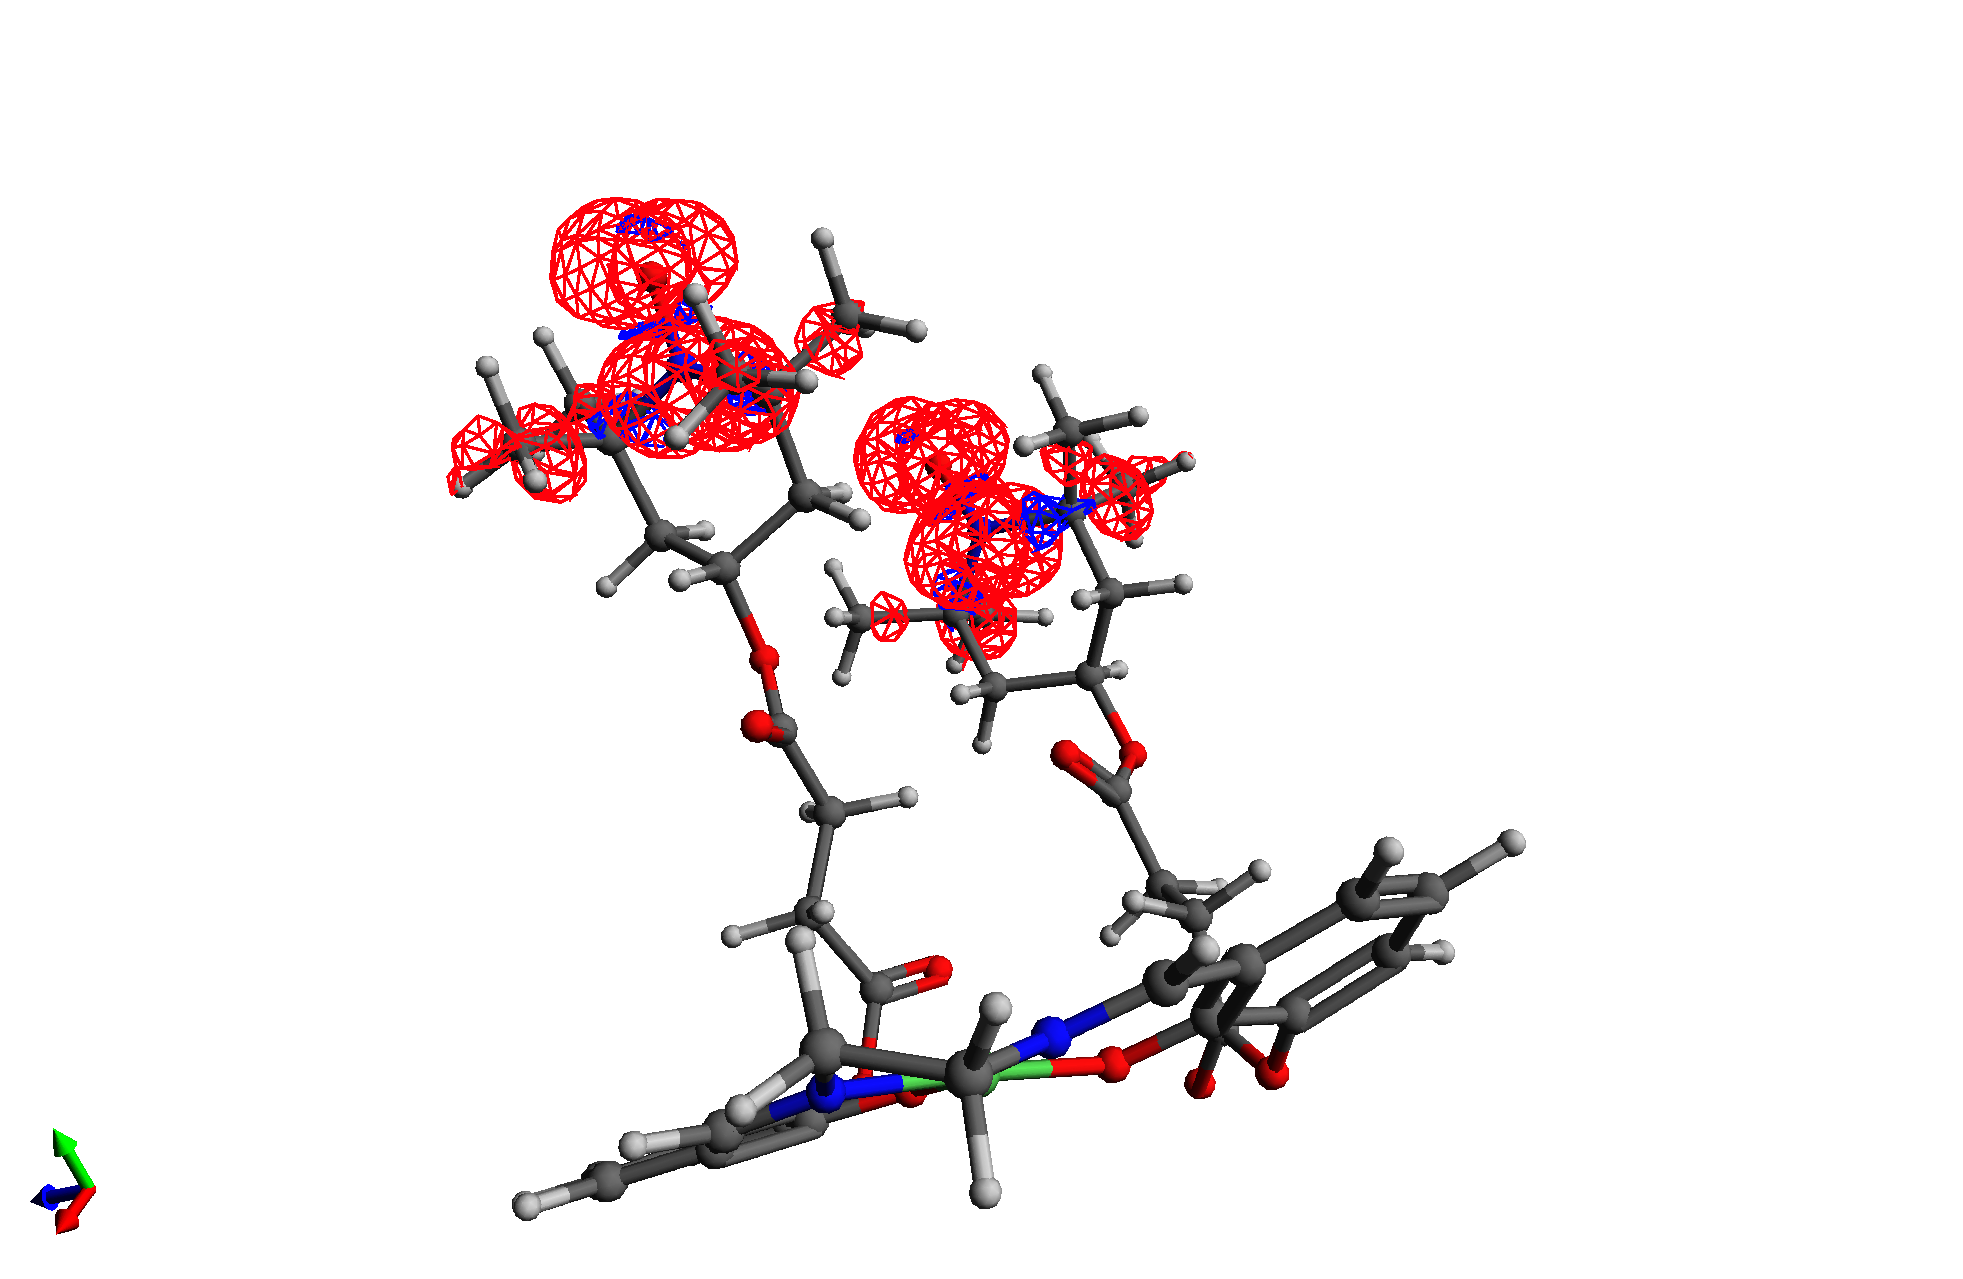
\includegraphics[width=1\textwidth]{./operando_epr/figures/DITS_DFT.pdf}
	\caption{Spin density in a DITS monomer with unoxidized TEMPO groups computed with density functional theory. The spin density localized on two neighboring TEMPO radicals, around the Nitrogen nuclei that gives rise to the hyperfine coupling. Calculation by Marcel Gauglitz in ORCA~\cite{Orca} at the high-performance computing cluster Curta of the Free University of Berlin~\cite{Curta}. The def2-TZVP functional basis set was used for the geometry optimization and for the calculations of the spin density.}
	\label{fig:TEMPO_dft}
\end{figure}



\subsection{Room Temperature Spectra of TEMPO$^{\bullet}$ Solutions}
Solution spectra of radicals are showing averaged values of $\textbf{g}$ and $\textbf{A}$ because of the fast molecular tumbling~\cite{Liu_2008,Carrington_solution_epr}. The observed $g$ value for a tumbling TEMPO$^{\bullet}$ is the average of the principal values of the $\textbf{g}$ matrix: $g = 1/3\left(g_{xx}+g_{yy}+g_{zz}\right)$. The anisotropic part of the hyperfine coupling tensor for the tumbling TEMPO$^{\bullet}$ also averages to zero, so only the isotropic hyperfine constant $a_{iso}$ determines the observed hyperfine coupling. CwEPR spectra of a 0.1~mM solution of TEMPOL measured at room temperature are shown in Figure~\ref{fig:cwEPR_monoTEMPO_diTEMPO_SOLUTION}. The spectral simulation performed with EasySpin~\cite{Stoll2006} yields $g=2.0055$ and $a_{iso}=43.8$~MHz.

\begin{figure}[h]
\center
	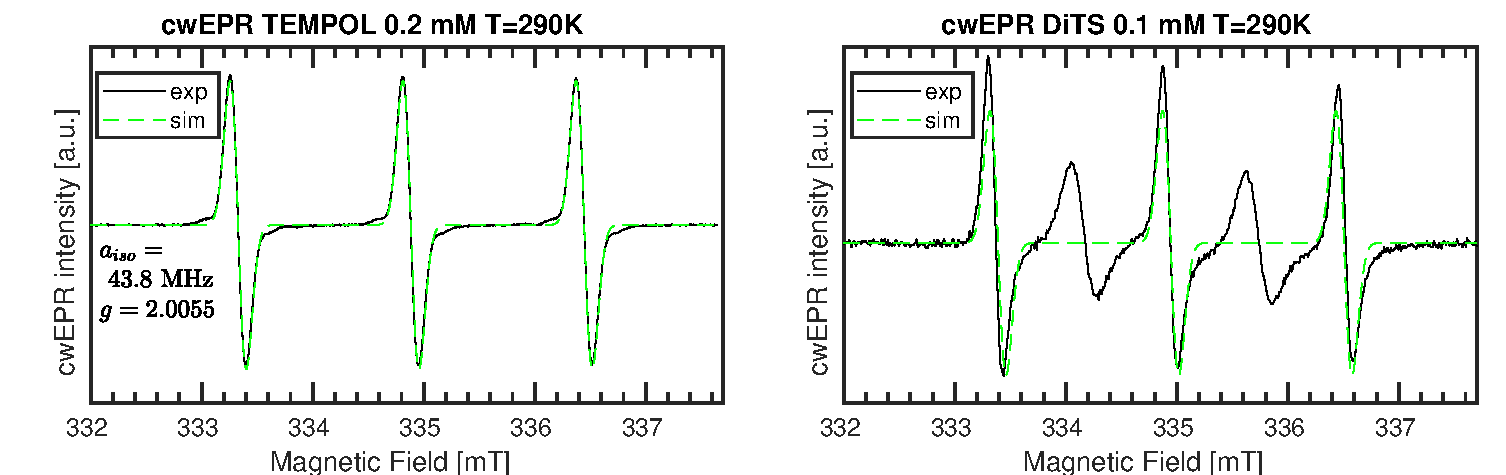
\includegraphics[width=1\textwidth]{./operando_epr/figures/TEMPOL/cwEPR_TEMPOL_vs_DiTS_RT.pdf}
	\caption{Room temperature cwEPR spectra of a low-concentration solutions containing mono- and di-TEMPO molecular fragments. Left: TEMPOL, three resolved spectral lines that correspond to the three hyperfine sublevels of $^{14}$N, equally separated by the isotropic hyperfine constant $a_iso$ Numerical simulations of the spectrum by varying $g$ and $a_iso$ parameters of the spin Hamiltonian and assuming fast molecular tumbling that averages $\textbf{g}$ and $\textbf{A}$ anisotropy. Lorentzian spectral profile due to the unresolved hyperfine couplings. Right: Di-Tempo-Salen. Three lines correspond to a mono-nitroxide spectrum, two additional broader lines appear due to the chemical exchange between the radicals at a rate comparable to the tumbling frequency.}
	\label{fig:cwEPR_monoTEMPO_diTEMPO_SOLUTION}
\end{figure}
\begin{figure}[h]
\center
	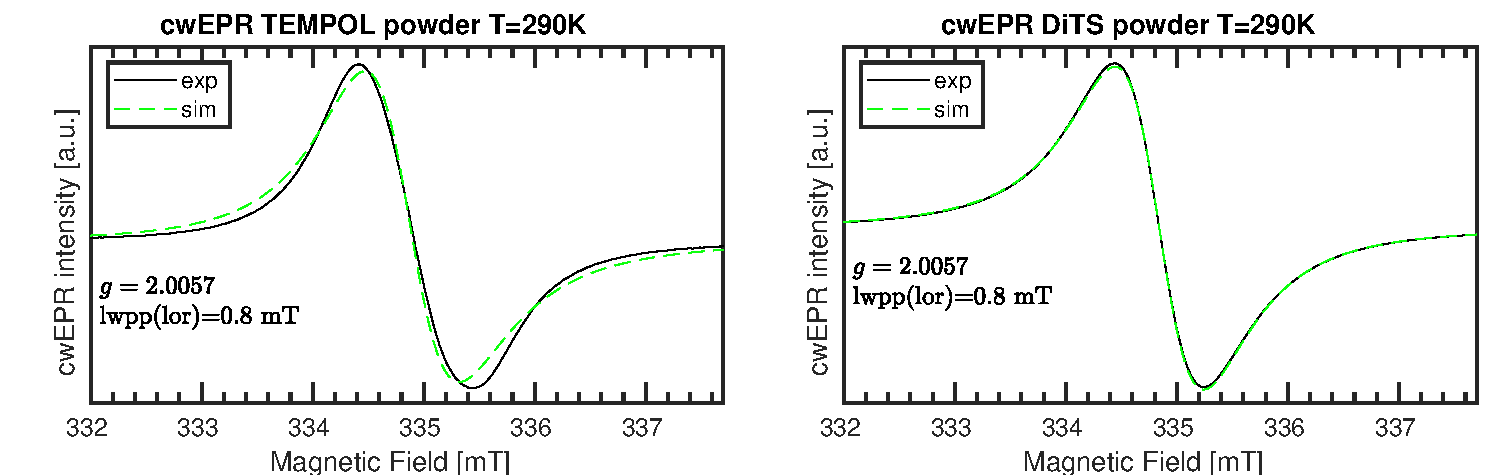
\includegraphics[width=1\textwidth]{./operando_epr/figures/TEMPOL/cwEPR_TEMPOL_vs_DiTS_RT_POWDER.pdf}
	\caption{Room temperature cwEPR spectra of pure TEMPO-containing powders. Left: TEMPO, Right: Di-Tempo-Salen. The strongly broadened lines represent significant dipolar couplings. Numerical simulations of the spectra by varying the isotropic $g$ value and the line width.}
	\label{fig:cwEPR_monoTEMPO_diTEMPO_POWDER}
\end{figure}

\begin{figure}[h]
\center
	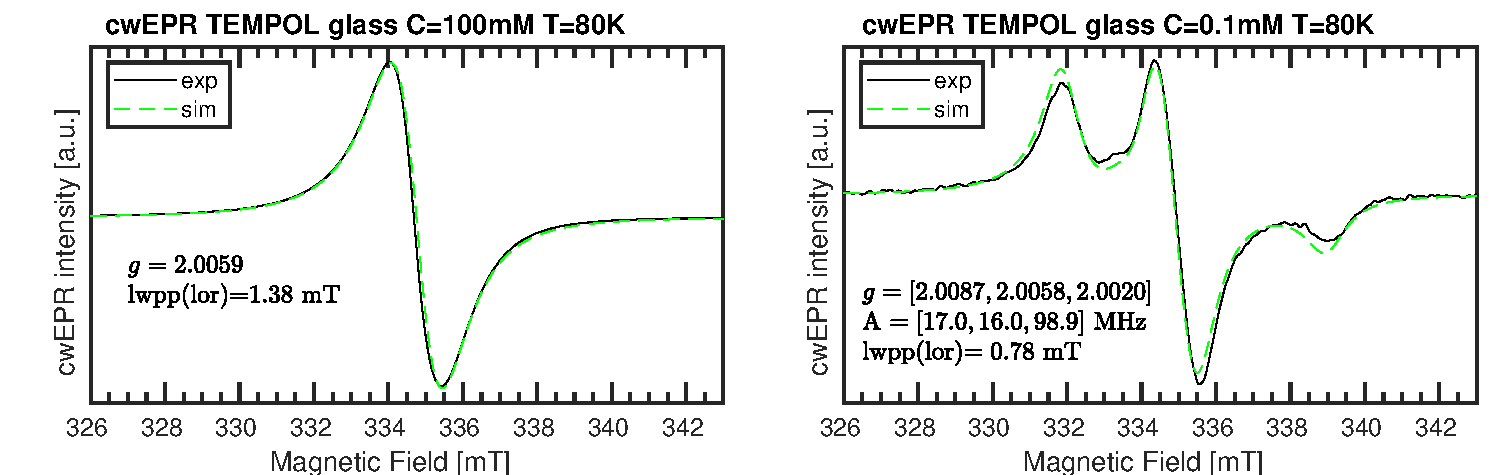
\includegraphics[width=1\textwidth]{./operando_epr/figures/TEMPOL/cwEPR_TEMPOL_100mM_vs_p1mM_80K.pdf}
	\caption{Cryogenic cwEPR spectra of TEMPOL at high and low concentration in a Dichloroethane/Acetonitrile glass. Left: 100~mM, Right: 0.1~mM. Numerical simulations of the spectra by varying $g$ and $A$ parameters of the spin Hamiltonian, as well as the line width.}
	\label{fig:cwEPR_TEMPOL_High_Low_Concentrations}
\end{figure}



\par
A biradical molecule like Di-Tempo-Salen (Figure~\ref{fig:molecules} e) and f) has two paramagnetic species that are close to each other and therefore exchange electrons. When the exchange coupling between the radicals $J$ is comparable to the hyperfine coupling $A$ of each radical to its 'host' nucleus, the superhyperfine interaction~\cite{Carrington_solution_epr} takes place, by which the radical is interacting to the nucleus of the neighboring radical~\cite{Eaton2018}. Solutions of biradical molecules with magnetic nuclei show more features in cwEPR spectra when the electron-electron exchange coupling $J$ between the two radicals within the molecule becomes comparable to the hyperfine coupling between the radical and its ``host'' $^{14}$N nucleus. tumbling of the molecule and the restricted motions of each radical within the molecule cause a complex molecular motion that affects the dipolar and exchange couplings between the radicals and causes ``spectra with alternating linewidths''~\cite{Eaton2018,Carrington_g_factor}. A solution of Di-TEMPO-Salen shows a five-line cwEPR spectrum with alternating linewidhts (Figure~\ref{fig:cwEPR_monoTEMPO_diTEMPO_SOLUTION}, right) with the three most intense lines corresponding to the three hyperfine sublevels of TEMPO$^{\bullet}$. The five-line structure in the cwEPR spectrum indicates the presence of a di-TEMPO biradical in the solution.\\
\newpage
.
\newpage
\subsection{Spectra of TEMPO$^{\bullet}$/TEMPO$^{+}$ Films}
\begin{figure}[H]
\center
	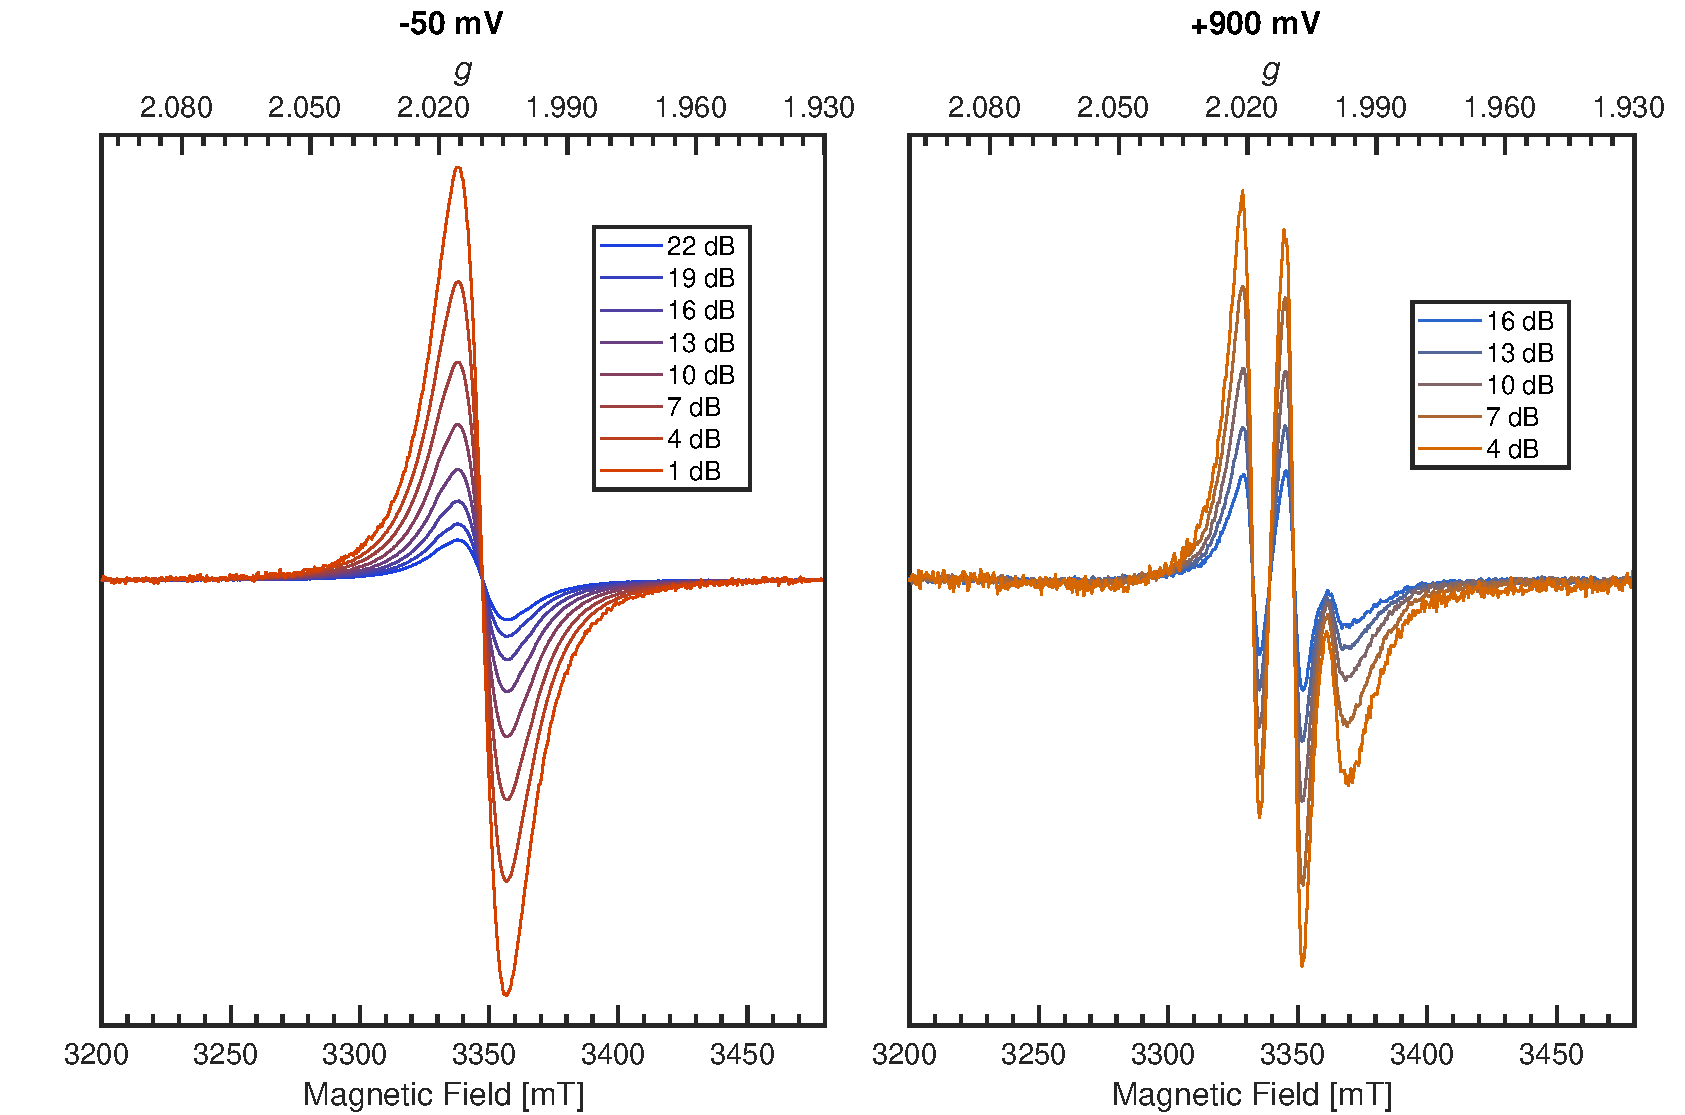
\includegraphics[width=1\textwidth]{./operando_epr/figures/CRYO/S220104_CW.pdf}
	\caption{Cryogenic (80~K) cwEPR spectra of a pDiTBuS film grown with 200 deposition cycles. Left: discharged film, -50~mV vs. Ag/AgNO$_3$ RE. Right: Fully charged film, 900~mV vs. Ag/AgNO$_3$ RE. Power series to detect possible microwave saturation. Microwave attenuation (dB) from 200~mW is shown in the legend.}
	\label{fig:cwEPR_CRYO_DiTBuS_DCG_vs_CHG}
\end{figure}
A film made of a TEMPO-containing polymer can be brought to a certain oxidation state, depending on how many of the TEMPO groups are in the radical (TEMPO$^{\bullet}$) state and how many are in the oxidized (TEMPO$^{+}$) state. The densely packed TEMPO$^{\bullet}$ fragments in the cathode film cannot be considered as isolated molecules anymore, and the interactions between the radicals become significant. Microcrystals of TEMPOL are densely packed TEMPO$^{\bullet}$ with a concentration of $4\times10^{21}~$cm$^{-3}=6900~$mM. The cwEPR spectrum of TEMPOL microcrystals in Figure~\ref{fig:cwEPR_monoTEMPO_diTEMPO_POWDER}, left is one broad line centered at $g=2.0055$. A powder of DiTS monomers is showing a similar cwEPR spectrum in Figure~\ref{fig:cwEPR_monoTEMPO_diTEMPO_POWDER}, right. It is the concentration of the peramagnetic TEMPO fragments that changes the cwEPR spectral shape. In Figure~\ref{fig:cwEPR_TEMPOL_High_Low_Concentrations}, left cryogenic (80~K) cwEPR spectrum of a 100~mM solution of TEMPOL in Dichloroethane/Acetonitrile is presented. With a slight shift in $g$ factor due to the polar molecular environment of the frozen solvent~\cite{Siavash} and a broader lineshape due to a weaker exchange narrowing, the spectrum consists on one dipolar-broadened Lorentzian line. In contrast, when the concentration of the solution is lowered to 0.1~mM (Figure~\ref{fig:cwEPR_TEMPOL_High_Low_Concentrations}, right) - the inter-molecular interactions become weak enough to resolve the $A$ and $g$ anisotropy of the nitroxide radical, so the spectrum consists of three lines that can be simulated with the known $\textbf{A}$ and $\textbf{g}$ parameters.\\
A redox-active film containing TEMPO radicals, like the TEMPO-Salen cathode film, shows different cwEPR signatures depending on its redox state. Figure~\ref{fig:cwEPR_CRYO_DiTBuS_DCG_vs_CHG} represents two crypogenic cwEPR spectra of a $d\approx2$~\SI{2}{\micro\meter} DiTBuS cathode film that was discharged to $E=-50$~mV and charged to $E=+900$~mV vs. the Ag/AgNO$_3$ RE as described in Section~\ref{sec:echem_charging}. The spectral intensities were normalized to represent the signal shape not the magnitude. The discharged film shows one broad cwEPR line in Figure~\ref{fig:cwEPR_CRYO_DiTBuS_DCG_vs_CHG}, left, that reflects on the strong interactions between the non-oxidized TEMPO$^{\bullet}$ in the discharged cathode. The linewidth of the discharged film spectrum is smaller than the linewidth of the DiTS monomer spectrum, suggesting a smaller exchange interaction between the TEMPO fragments in the film~\cite{Vereshchagin2020}.\\
The oxidized film in Figure~\ref{fig:cwEPR_TEMPOL_High_Low_Concentrations}, right, shows a well resolved spectrum of an isolated nitroxide, similar to the low-concentrated solution of TEMPOL (Figure~\ref{fig:cwEPR_TEMPOL_High_Low_Concentrations}, right). A series of powers was recorded for both redox states of the film to observe possible microwave saturation effects that are crucial for the pulsed EPR experiments discussed in Chapter~\ref{ch:pulsed_epr}. The microwave saturation happens when the (cw) microwave power is sufficiently high to excite the $\vert{\downarrow}\rangle-\vert{\uparrow}\rangle$ transitions in the sample at a rate that is faster than the spin relaxation times. Microwave saturation leads to a weaker absorption, hence a weaker cwEPR signal at a certain microwave power level. In the range of microwave powers where no saturation takes place, the cwEPR intensity is proportional to the amplitude of $B_1$, that is, without saturation, the cwEPR intensity increases linearly as a function of the square root of the microwave power~\cite{Eaton_book}. For both SoC, the cwEPR intensity of the pDiTBuS film doubles when the microwave power is increased by 6~dB, so no saturation is seen for both states of charge in the used range of the microwave power. This indicates that the relaxation times in the cathode film are rather short, both for charged and uncharged states. The 0-dB power of the used cwEPR microwave bridge was 200~mW.
\begin{figure}[]
\center
	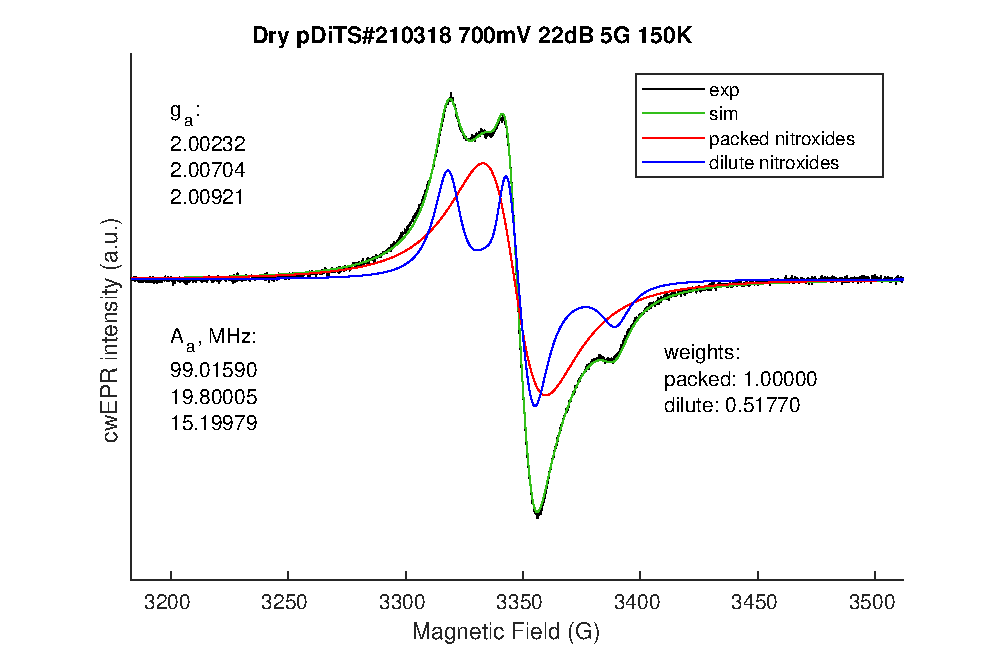
\includegraphics[width=0.8\textwidth]{./operando_epr/figures/CRYO/cw_sim_pDiTS_210318_700mV_2comp.pdf}
	\caption{A pDiTS film in the intermediate state of charge (700~mV vs. Ag/AgNO$_3$) showing a composition of two spectral signatures. The single-line signal from the densely packed nitroxide radicals coexists with the signal of the isolated nitroxide radicals. Two-component simulation.}
	\label{fig:cwEPR_CRYO_DiTS_2_COMP_SIM}
\end{figure}
\begin{figure}[h]
\center
	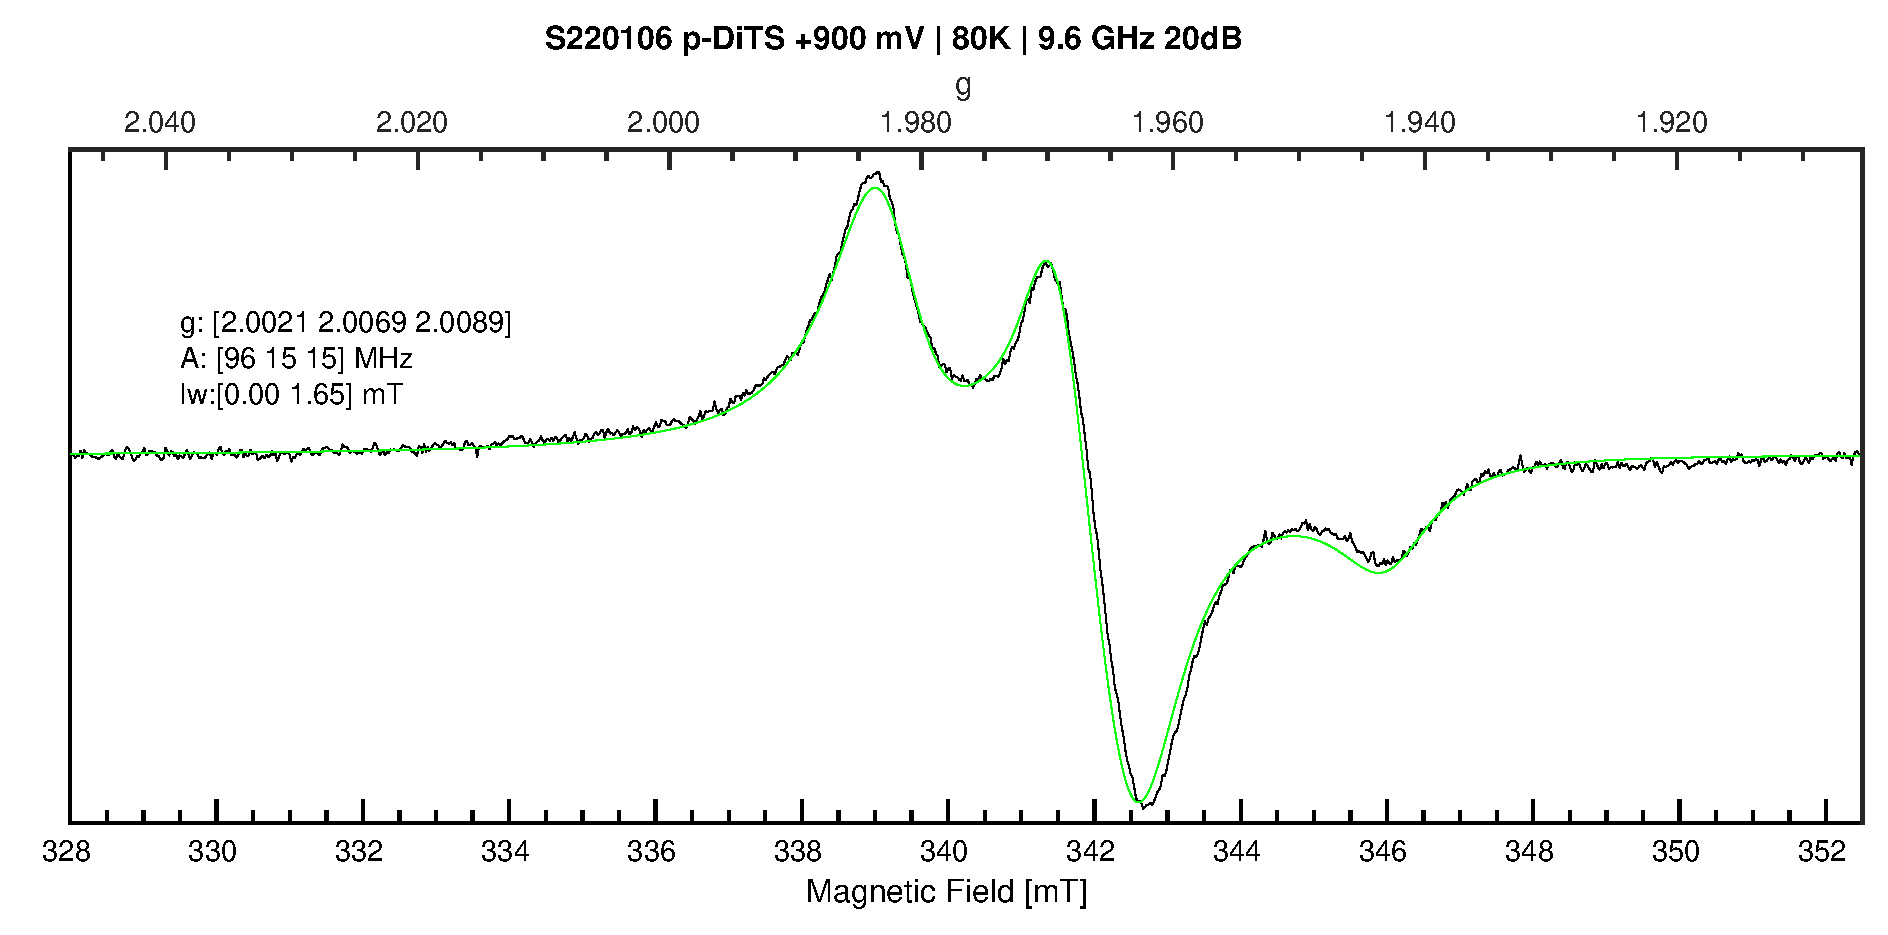
\includegraphics[width=0.9\textwidth]{./operando_epr/figures/CRYO/S220106_p-DiTS_OX_80K_CW_SIM.pdf}
	\caption{Cryogenic (80~K) cwEPR spectrum of a strongly oxidized ($E=900$~mV vs. Ag/AgNO$_3$) pDiTBuS film grown with 200 deposition cycles showing a signature of the isolated nitroxide radical with the standard $g$ and $A$ parameters, revealed with a numerical simulation with EasySpin~\cite{Stoll2006}.}
	\label{fig:cwEPR_CRYO_DiTBuS_CHG_SIM}
\end{figure}



\begin{figure}[h]
\center
	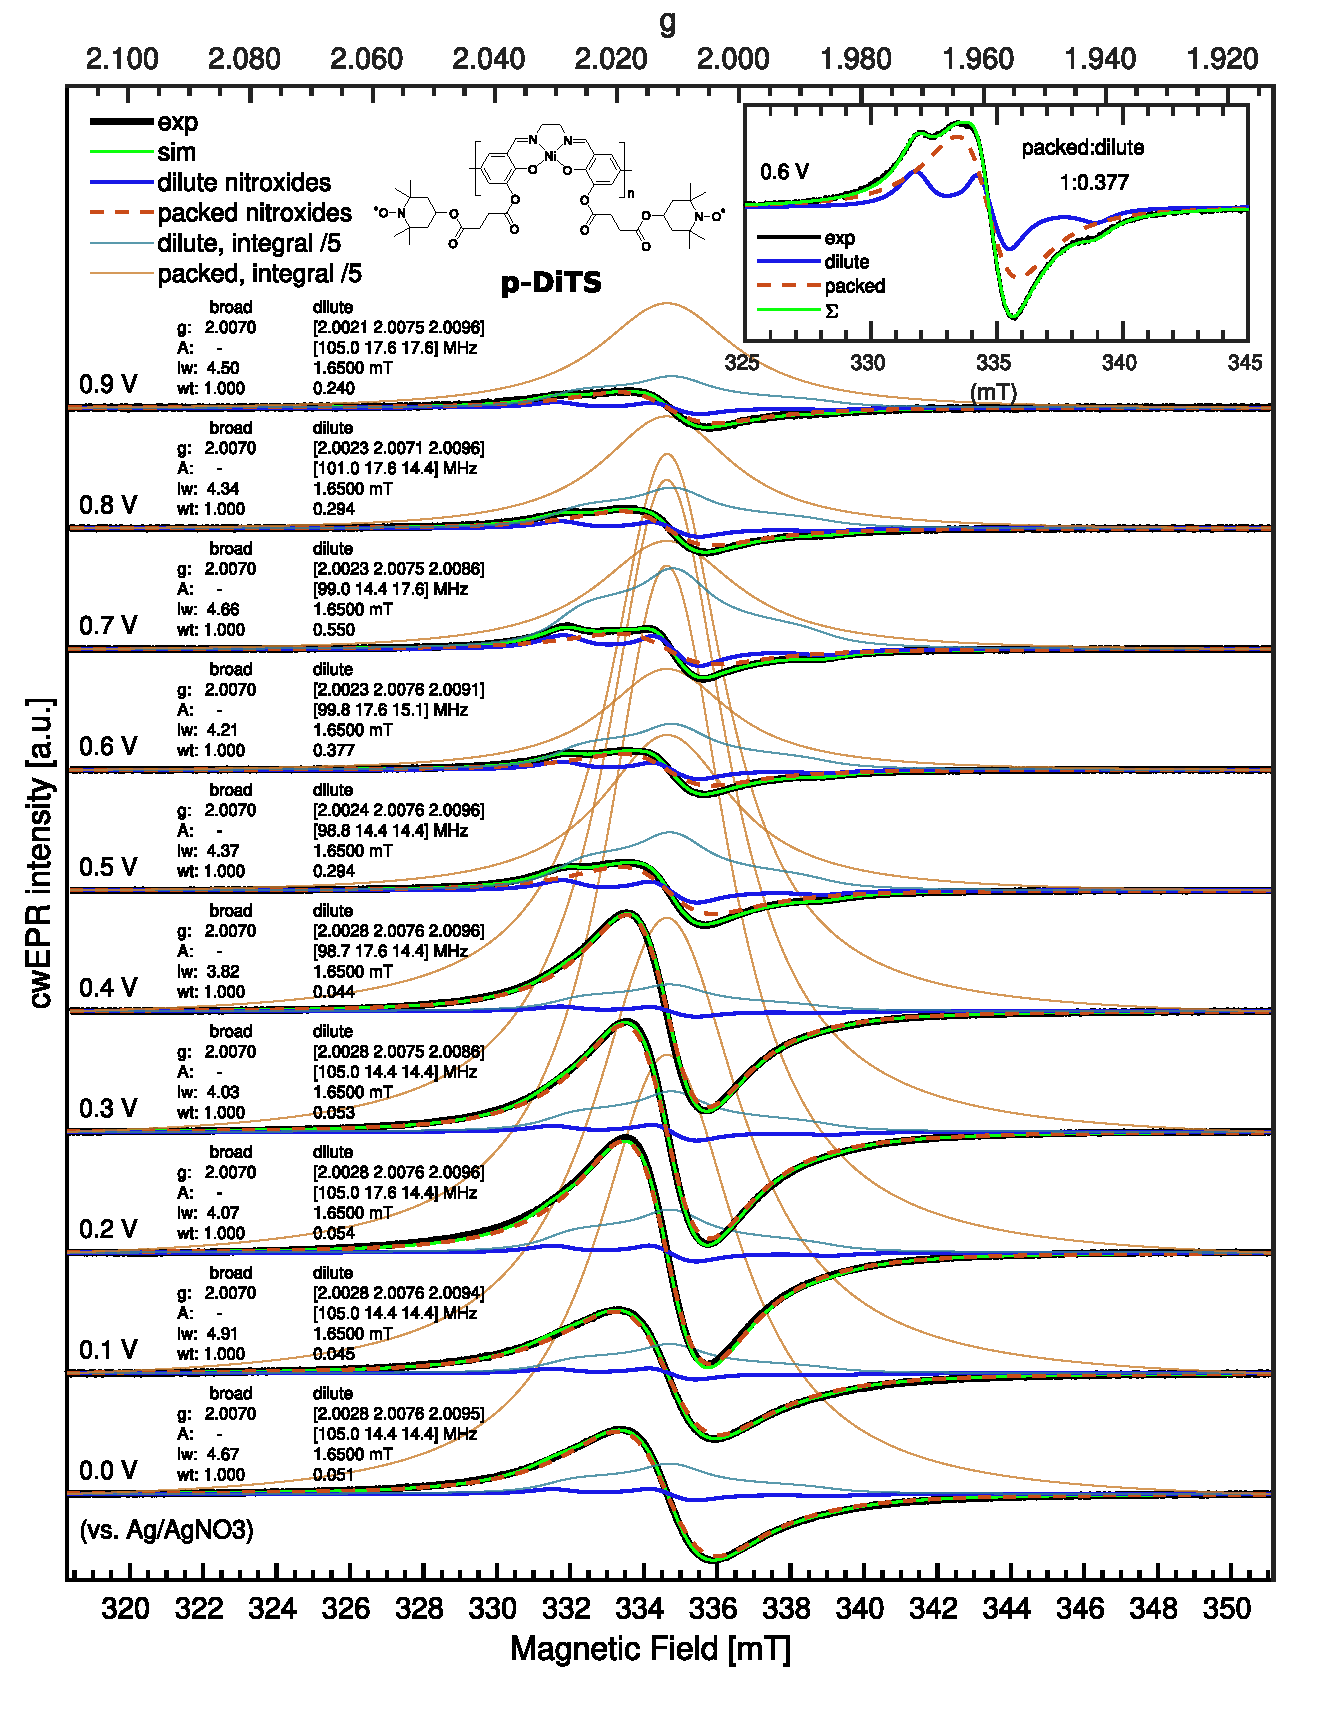
\includegraphics[width=1\textwidth]{./operando_epr/figures/CRYO/Figure_S7_new.pdf}
	\caption{Ex-situ SEC cwEPR measurements ($\nu=$9.4~GHz) on a dry p-DiTS film at 150~K. Decomposition of spectra into two components with numeric simulations using EasySpin~\cite{Stoll_2006}: a broad Lorentzian line (g = 2.0070, lw = 4.63$\pm$1.00~mT) and a dilute component with a hyperfine coupling to $^{14}$N ($I$ = 1, $g$ = [2.00231 2.00711 2.00912], $A$ = [100 15 15]$\pm$5 2 2]~MHz, Lorentzian broadening with lw = 1.65~mT). The absorption profiles are shown with the integrals of the EPR signals. The ratio between the simulated components for each potential is shown by the double integrals of the components. Inset: sum of the broad and dilute components that reproduce the line shape at 0.6~V.\\}
	\label{fig:cwEPR_CRYO_DiTS_CHG_SIM}
\end{figure}

\newpage
.
\newpage
.
\newpage

\subsection{Characteristic cwEPR Spectra of a TEMPO-Salen Cell}

\begin{figure}[H]
\center
	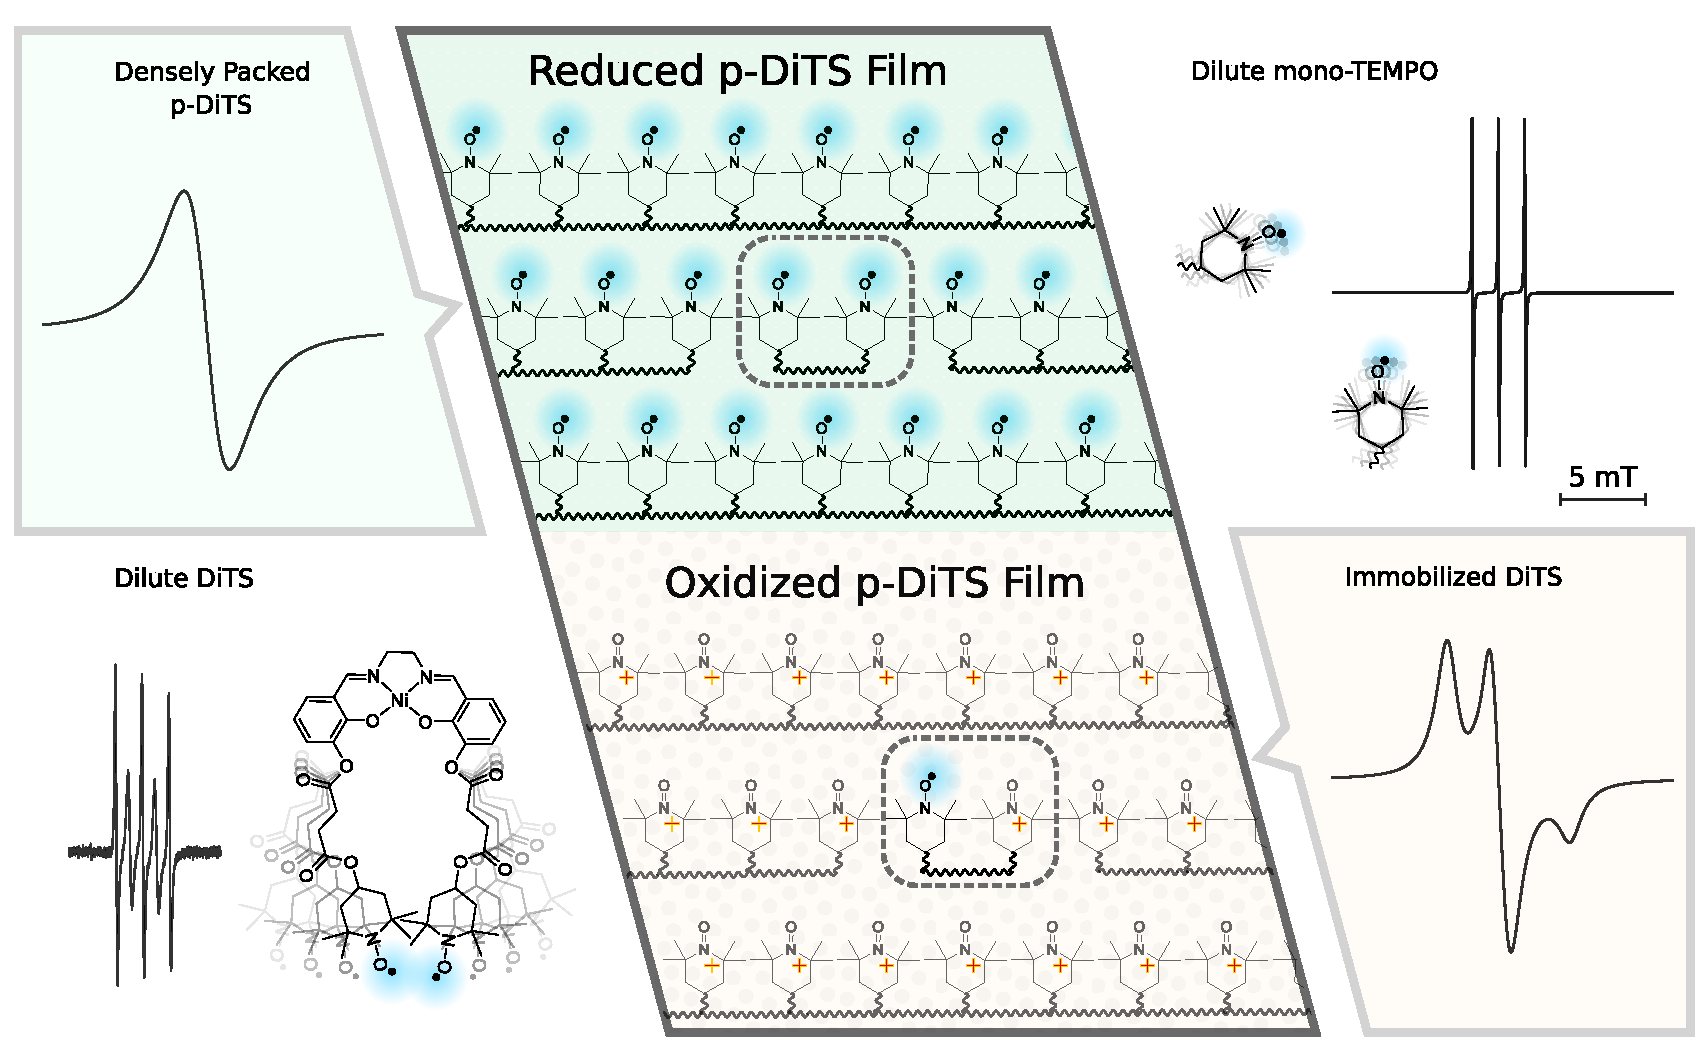
\includegraphics[width=1\textwidth]{./operando_epr/figures/Cartoon_ALL.pdf}
	\caption{Classification of the nitroxide cwEPR spectra observed for p-DiTS under different conditions and in different environments. a): Densely packed nitroxide film with dipolar broadening and exchange narrowing or broadening giving a single derivative line. b): Typical spectrum of a dilute mono-nitroxide in solution, three-lines due to $S=1/2$, $I=1$ $^{14}$N hyperfine interaction (described by isotropic $g$-factor and isotropic hyperfine ($A$) interaction). c): Typical spectrum of a tumbling di-nitroxide in solution where dynamic changes in the nitroxide -- nitroxide distance modulate the exchange interaction yielding a five-line structure with alternating line width (measured cwEPR of DiTS monomers in solution at room temperature). d): Immobilized nitroxide spectrum with both $g$ and $A$ anisotropy.}
	\label{fig:cartoon_spectra_dts}
\end{figure}

There are four characteristic cwEPR signatures of an electrochemical cell containing di-TEMPO-Salen polymer cathode. The well known signature of a freely tumbling TEMPO$^{\bullet}$ exhibits three narrow lines corresponding to the three nuclear sublevels of nitrogen: $m_I=-1,0,+1$.\\

EPR spectra of electrochemical cells with p-DiTS as active-electrode material can exhibit a variety of different signals. Before presenting and discussing the experimental results, we will provide an overview about the various characteristic cwEPR lineshapes associated with nitroxides in different environments.
\par

Fig.~\ref{fig:cartoon_spectra_dts}a shows the spectrum expected for a \emph{densely packed p-DiTS film} with all nitroxides in the EPR-active reduced state. The broad unstructured line results from the strong dipolar and exchange interaction between both nitroxides of each DiTS monomer as well as between the nitroxides of different monomers. The exchange interaction can lead to either line narrowing or broadening depending on the strength of the interaction~\cite{Anderson1953}, while the dipolar interaction causes broadening. In consequence, the overall cwEPR line width depends on the spin concentration in the film.
\par 
\emph{Dilute mono-TEMPO fragments} dissolved in the electrolyte, each containing only one nitroxide, give rise to a three-line spectrum (cf.\ Fig.~\ref{fig:cartoon_spectra_dts}b) which is well known from nitroxide-based spin labels in solution.\cite{Liu_2008} Tumbling of the molecules in the liquid electrolyte results in an averaging of the anisotropic interaction between the electron spin and the nitrogen nuclear spin ($I = 1$) as well as of the $g$ anisotropy, leaving only the isotropic part of the hyperfine coupling and the isotropic $g$ value. 
\par
\emph{Dilute DiTS monomers} in the electrolyte generally give a spectrum consisting of five narrow lines (cf.\ Fig.~\ref{fig:cartoon_spectra_dts}c), if each monomer contains two interacting EPR-active nitroxides. The spectrum depends on dynamic effects, specifically the modulation of the exchange interaction between both radicals of each monomer.  Thus, depending on the solvent and temperature, the spectrum can be indistinguishable from the three-line spectrum of mono-TEMPO fragments.
\par
The fully charged (oxidized) p-DiTS film can contain electrically isolated domains in which the nitroxides are not connected to the electrode and cannot be oxidized or reduced. These electrically inactive \emph{immobilized DiTS monomers} in the oxidized film display a spectrum as shown in Fig.~\ref{fig:cartoon_spectra_dts}d. In contrast to the densely packed p-DiTS film, the dipolar and exchange interactions between neighboring radicals are much weaker. The anisotropy of the nitroxide's hyperfine tensor adds features to the cwEPR spectrum in d) as compared to a).
Yet, there is some remaining line broadening that does not allow one to distinguish between immobilized DiTS monomers with either one or two paramagnetic nitroxides.
\par
We note that the oxidized NiSalen backbone can contribute to the spectrum as well. Its EPR signature, which is not shown in Fig.~\ref{fig:cartoon_spectra_dts}, is clearly different from the nitroxide/TEMPO-related spectra discussed above.
%

\subsection{cwEPR Spectra During a Charge--Discharge Cycle}
\label{sec:operando_dits}

\begin{figure}[H]
\center
	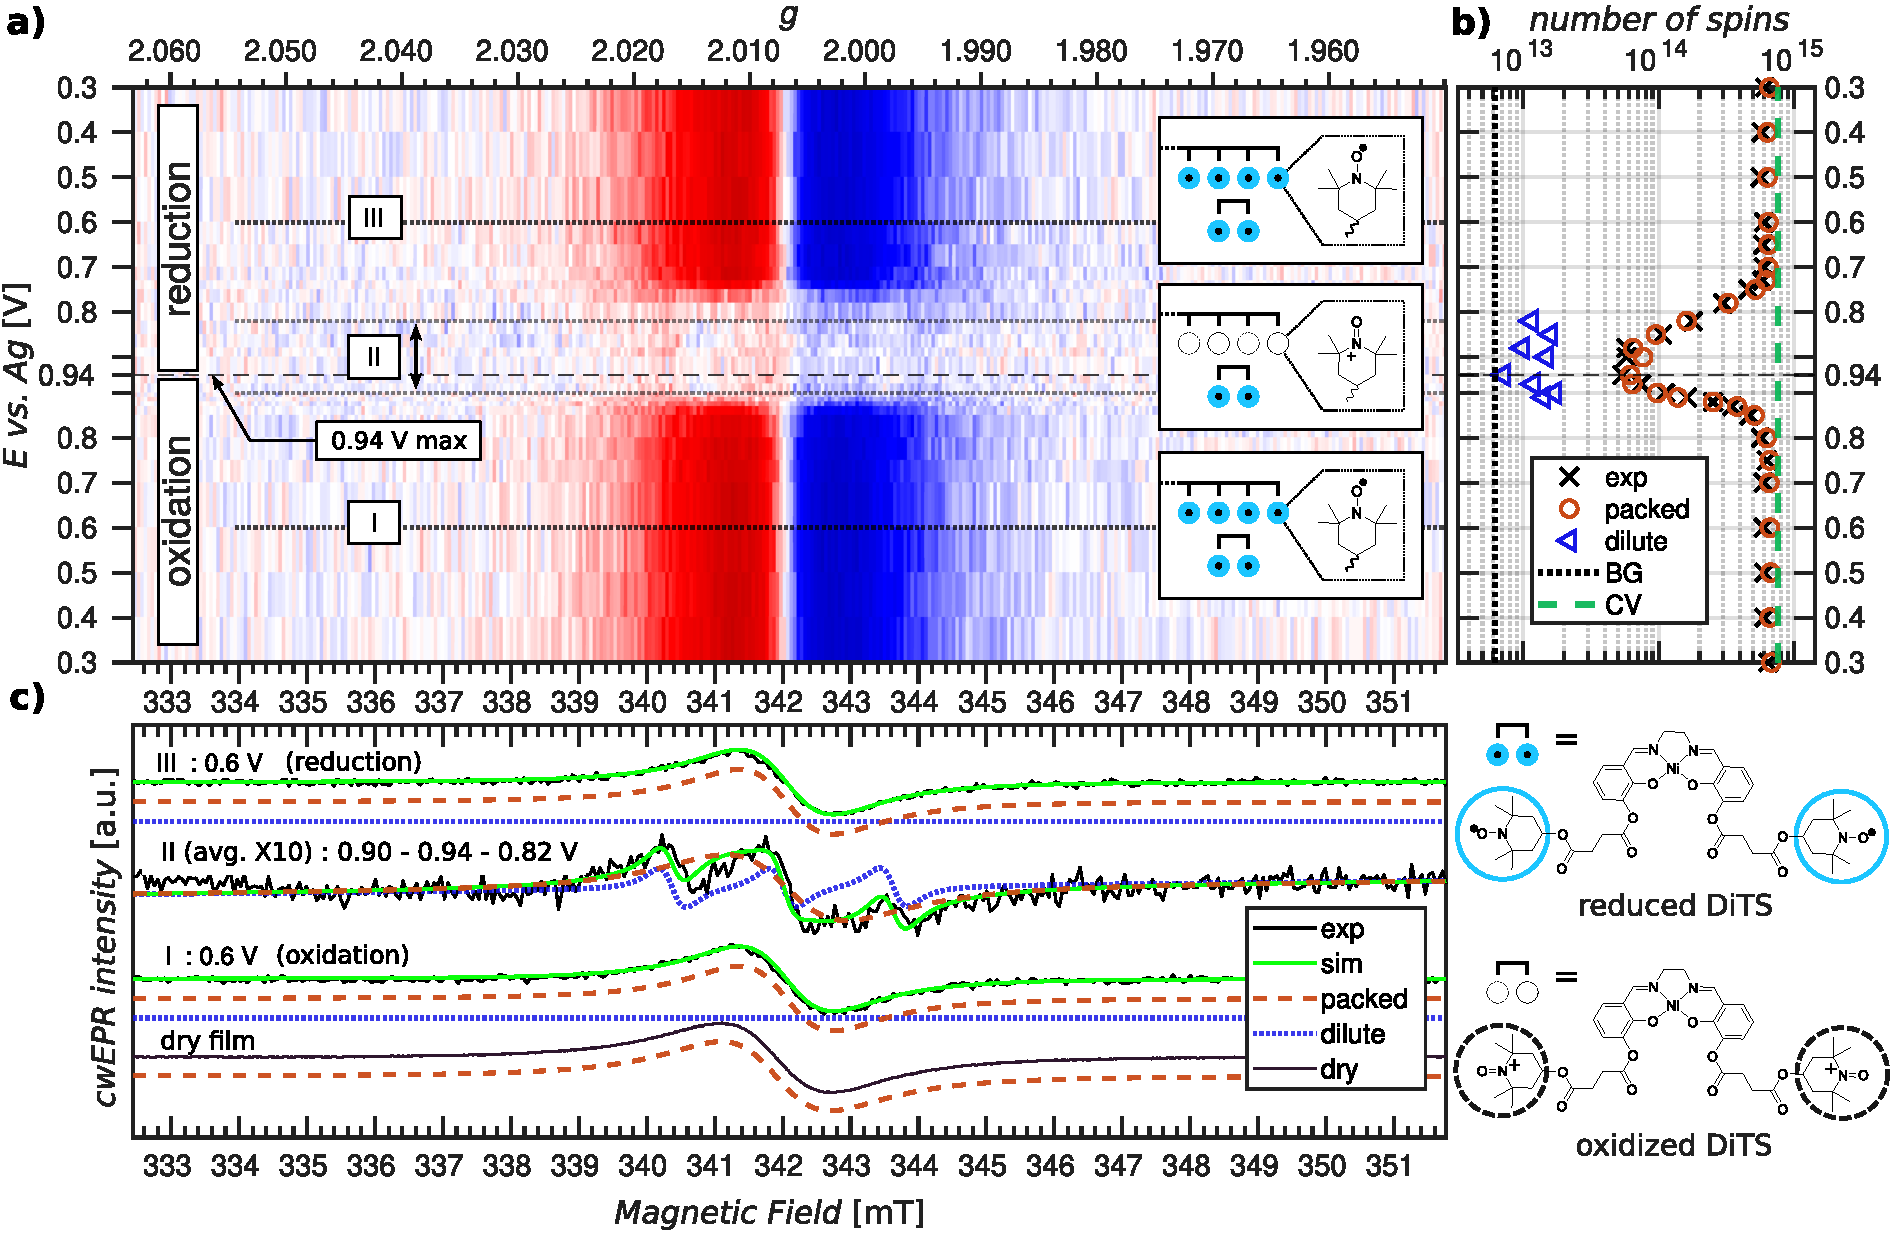
\includegraphics[width=1\textwidth]{./operando_epr/figures/Main_2D_redox_map_full.pdf}
	\caption{Room-temperature in-operando cwEPR for a p-DiTS electrochemical cell ($\nu = 9.6$~GHz). a): CwEPR spectra during charging (oxidation) and discharging (reduction) of the cell. b): Number of unpaired electron spins determined from a quantitative analysis of the spectra (exp). Deconvolution of the total spin count into packed and dilute spectral components. Number of electrochemically active electrons in the p-DiTS film determined from its cyclic voltammogram. Background spin count on a cell without the p-DiTS film (BG). c): Slices of subplot a) for the initially discharged state (\RomanNumeralCaps{1}, 0.6~V), charged state (\RomanNumeralCaps{2}, 0.90--0.94--0.82~V, averaged within the region denoted by $\updownarrow$~, scaled up $\times$10), and the final discharged state (\RomanNumeralCaps{3}, 0.6~V). Two-component spectral simulations to identify the contributions of dilute and packed nitroxide fragments at each potential. Potentials were recorded vs.\ Ag RE.}
	\label{fig:operando_carpet}
\end{figure}


In this section the cwEPR spectra are presented at each measured potential during the in-operando redox series for a p-DiTS film deposited with 8 electro-polymerization cylces ($t=$~40~nm). The experimental data are fit with two components. Component 1 describes the densely packed immobilized nitroxide spins and component 2 describes the dilute mobile nitroxide spins in the electrolyte. All simulation parameters and relative weights of the two components are shown in Fig.~\ref{fig:S4}.\\

\newpage
\begin{figure}[H]
\centering
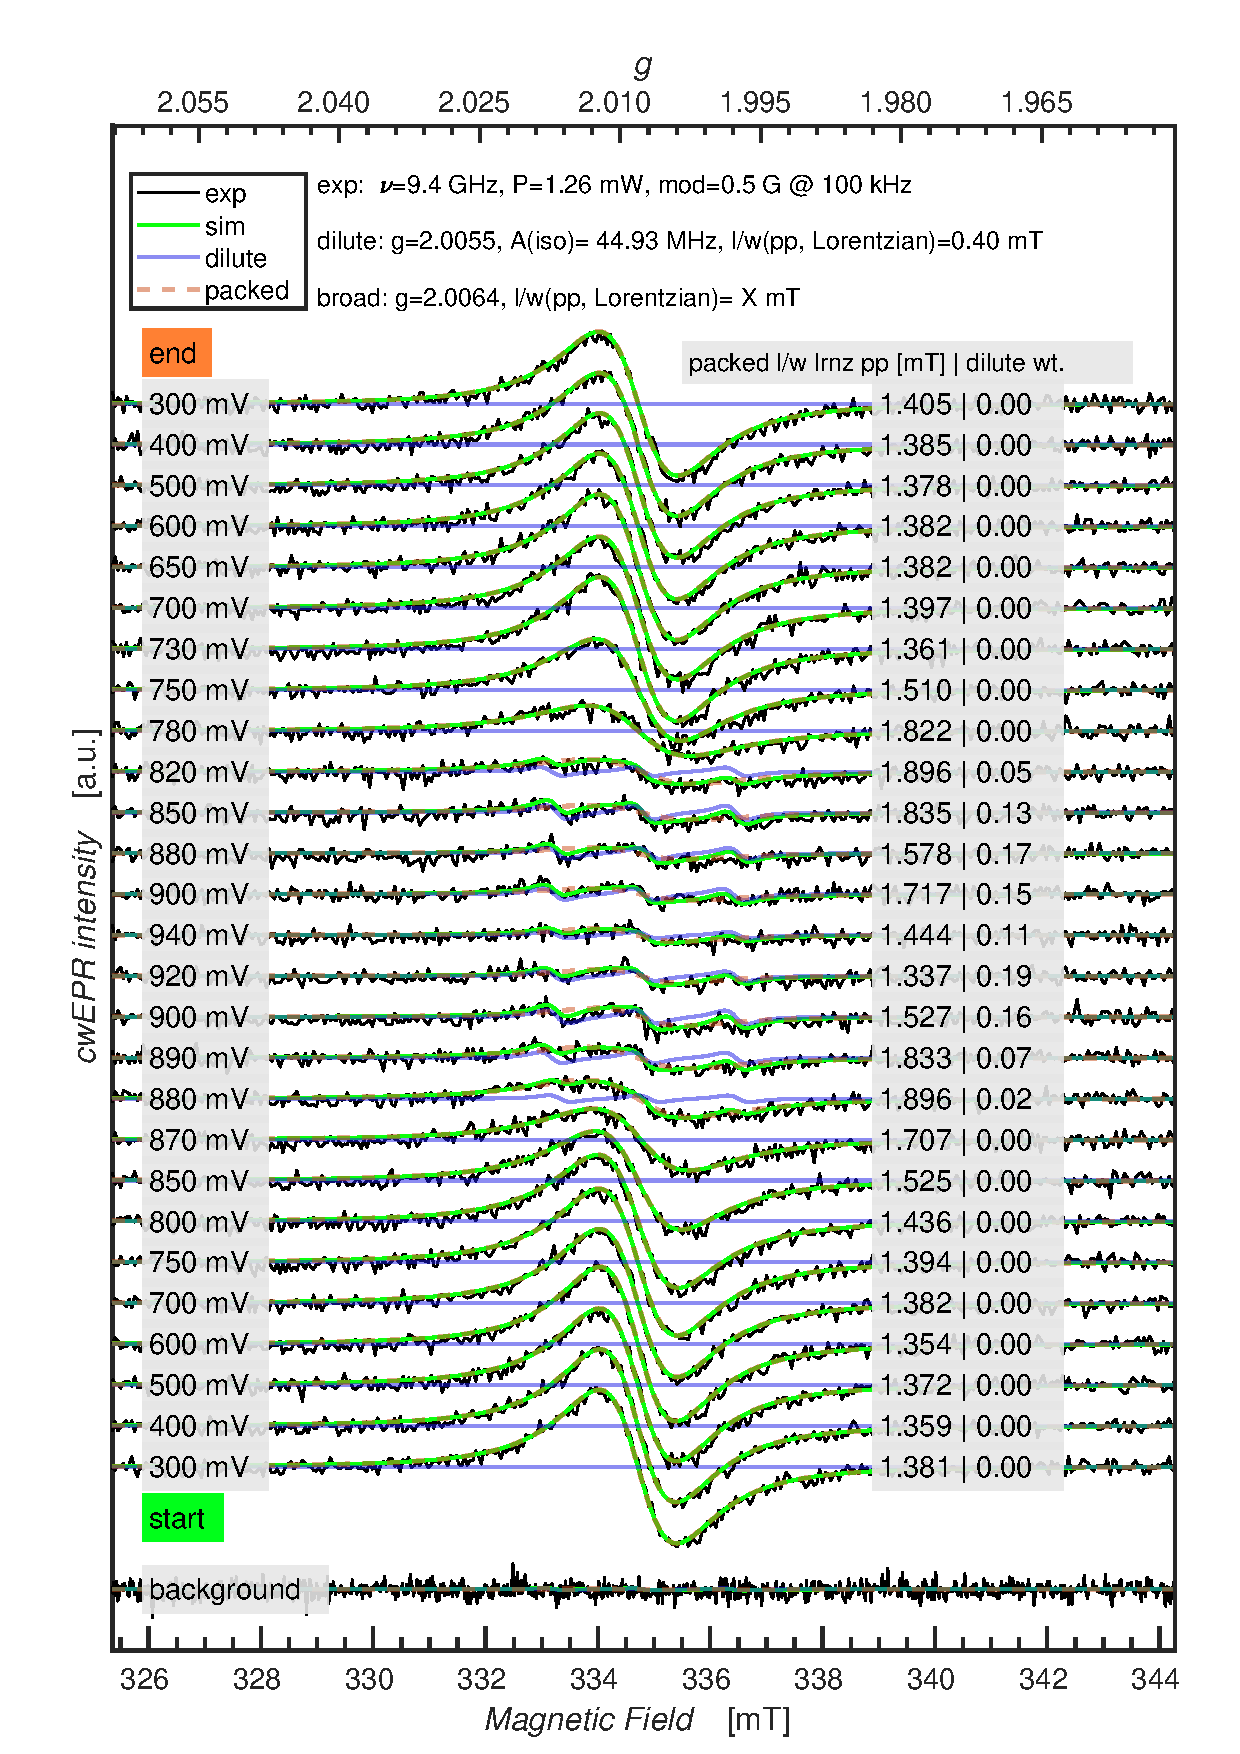
\includegraphics[width=0.94\textwidth]{./operando_epr/figures/Figure_S4}
\caption{Room temperature in-operando SEC cwEPR on a 8-CV p-DiTS film. $\nu=$~9.4~GHz. black - experimental spectra, green - simulation consisting of two components with relative weight as shown in the plot, dashed-red - component 1 the coupled spins in the film, blue - component 2 the dilute mobile spins in electrolyte. All simulation done using Easyspin~\cite{Stoll2006}.}
\label{fig:S4}
\end{figure}

Potential dependent in-operando SEC cwEPR was measured on a 40$\pm$5~nm thick (8 deposition cycles) p-DiTS film inside the modified EPR tube at room temperature (see Fig.~\ref{fig:operando_carpet}). At 0.3~V (vs. Ag) the TEMPO fragments are in the reduced/discharged state. The discharged film exhibits a single Lorentzian derivative lineshape with a peak-to-peak line width of 1.4~mT. The single-line derivative lineshape results from the collapse of the hyperfine structure due to strong exchange coupling in the films with high spin concentration, whereas the broader line width is due to a combination of dipolar and exchange coupling between the nitroxide spins within the film. In this reduced, neutral radical state the number of unpaired electrons in the film was calculated to be $6\times10^{14}$ (with up to 20\% error in quantitative cwEPR). This is comparable to the number of electrochemically active TEMPO charges at $8\times10^{14}$, determined by integration of the reduction branch of the CV of the cell vs.\ time.
\par
Upon increasing the oxidation potential, there is no significant change in the cwEPR spectra in the oxidation potential range between 0.3~V and $\sim$0.8~V (region~I). A representative cwEPR spectrum from region~I, taken at an oxidation potential of 0.6~V, is shown in Fig.~\ref{fig:Figure_4}c, where the peak-to-peak line width is 1.4~mT. There is no significant change in the number of spins (spin count) contributing to the cwEPR spectra at all potentials in region~I, as shown in Fig.~\ref{fig:Figure_4}b. The cwEPR signal intensity starts to decrease at 0.8~V, and from 0.85~V to 0.94~V (the maximum potential applied to this cell), the signal intensity drops sharply. The lowest spin count is observed at an oxidation potential of 0.94~V giving $5\times10^{13}$ spins. This is an order of magnitude decrease in the number of unpaired electrons in the oxidized film as compared to its initial, reduced state.


\par
Upon closer inspection, by averaging the cwEPR spectra in oxidized region II (between the potentials of 0.90 -- 0.94 -- 0.82~V), one clearly sees that the spectral shape has substantially changed from the initial region I spectrum. The region II averaged spectrum can be decomposed into two spectral components (see Fig.~\ref{fig:Figure_2}c) by simulating the spectra with the MATLAB toolbox EasySpin~\cite{Stoll2006} (``garlic'' function). Component 1 (``packed'') is again a broad Lorentzian derivative, similar to that of region I, but with an increased line width of 1.8~mT. Component 2 (``dilute'') is a fast-motion spectrum of tumbling nitroxides.

\par
The presence of component 1 even at the oxidation potential of 0.94~V is at first unexpected, as at this potential the CV curve shows full TEMPO oxidation (cf.\ Fig. \ref{fig:Figure_1}e for a representative CV in a tube for p-DiTS). We therefore suggest that component 1 corresponds to local islands of still densely packed spins, which are electrically disconnected from the rest of the film (and the electrodes) and hence not redox active. The line width of component 1 in region II at 1.8~mT is slightly broader than in region I, suggesting a change in the spin-spin couplings. Looking at the line width of component 1 at different oxidation and reduction potentials (cf.\ Fig.~\ref{fig:S4}, ESI$\dag$), we clearly see a trend in that the line width increases from $\approx$~1.3--1.4~mT in the beginning of region I to $\approx$~1.8~mT by the end of region I, at 0.9~V. The reverse is true for region III, where the line width decreases from $\approx$~1.8~mT at 0.9~V back to $\approx$~1.3--1.4~mT at 0.3~V. Since the dipolar coupling between the spins should only decrease with increasing potentials (reducing spin count in the film) resulting in a decreasing line width, we expect the observed line width behavior (increasing line width when going from 0.3~V to 0.9~V) to be due to decreasing exchange coupling. As the film is oxidized, the spin density in it decreases. That reduces the exchange coupling between neighboring spins, which transforms an exchange narrowed spectrum (strong exchange coupling) into an exchange broadened spectrum (weaker exchange coupling). However, the spin concentration in the film cannot be decreased to a point where the hyperfine structure can be resolved.

\par
Furthermore, since the component 1 spectra in region II are likely to be due to local islands of electrochemically inactive charged species, their spectral line width depends on the local spin concentration before the charges/islands become electrically inactive. It is unclear why the line width observed for component 1 is larger in region II, though possible reasons are weak cwEPR signals introduce a systematic error into the two-component spectral deconvolution, or the exchange narrowing effect is less pronounced at the decreased spin concentration, or there is a changing morphology during oxidation. The idea of electrically disconnected islands or domains will be further explored later on in Section~\ref{Degradation_study}.

\par
The presence of component 2 (three-line feature described by an isotropic $g$-factor and hyperfine interaction) is, as discussed in Section \ref{Classification}, due to mobile nitroxide spins. The presence of a three-line component but no detectable five-line component suggests the nitroxide spins in electrolyte are not due to the release of monomers (as expected for this film because it underwent the cleaning procedure described in Section \ref{CVTube} to remove any non-polymerized DiTS). The three-line feature must therefore be due to molecular breakdown of DiTS to release mono-nitroxide fragments in the electrolyte.

\par
We determine the spin counts for the components 1 and 2 by double integration of the simulation traces around 0.94~V. Component 1, the packed immobilized nitroxide spins, corresponds to a spin count of $4.8\times10^{13}$ at 0.94~V (Fig.~\ref{fig:Figure_4}b, orange circles), while component 2, the dilute mobile nitroxide spins in electrolyte, corresponds to $\approx 1\times10^{13}$ (Fig.~\ref{fig:Figure_4}b, blue triangles). The number of spins due to nitroxide groups dissolved in the electrolyte is only $\sim$1.6~\% of the total spins in the initial film (cf.\ total initial spin count of $6.4\times10^{14}$). The number of nitroxide spins, which are still part of the film but not oxidized, is only $\sim$7.5~\% of the initial spin count. This shows that over 90\% of the p-DiTS film is electrochemically active.

\par
Looking at the oxidation series from 0.3~V to 0.94~V and the reduction series from 0.94~V back to 0.3~V, we see that the reduction occurs over a larger potential range as compared to the oxidation (cf.\ Fig.~\ref{fig:Figure_4}b). This suggests a changing morphology of the p-DiTS film upon oxidation, which decreases electrolyte access to the TEMPO groups in the film matrix. A similar trend is seen in thicker films, where again oxidation occurs over a narrower potential range than reduction (see Fig.~\ref{fig:S6}, ESI$\dag$). This is a known phenomenon whereby, during oxidation, the pores and channels in the polymer film open and counter ions from the electrolyte enter the film matrix, aiding the oxidation process. During reduction, the opposite is true whereby the polymer film shrinks, and hence expulsion of counter ions slows down as a function of time. This results in a broadening of the left-hand side of the reduction branch in a CV and a slower recovery of the TEMPO spin count during the reduction series in quantitative in-operando cwEPR. 

\par
While the EPR signatures of different polymeric NiSalen complexes have been reported by Dmitrieva \textit{et al.},\cite{Dmitrieva2018} we do not observe the EPR signature of the NiSalen backbone in our in-operando study of p-DiTS. Dmitrieva \textit{et al.}\ noted that upon increased doping of the polymer (still one electron per monomer unit), the charges could aggregate to form diamagnetic states, and under high oxidation potentials the polymer could be doped with two electrons per monomer, thus also forming diamagnetic dications. Another plausible explanation for the absence of a p-NiSalen EPR signal could be related to low-intensity signals which are masked by the much more intense nitroxide signals. However, our quantitative EPR analysis of the number of spins per monomer unit in this film gave 2.0$\pm$0.2, suggesting only signals corresponding to nitroxide radicals, as there are two unpared nitroxides per DiTS monomer unit: in its charge-bearing groups.
In addition, Coulomb repulsion between the positively charged TEMPO$^+$ groups in the oxidized state and the positive polarons on the backbone could lead to a depletion of mobile positive charge carriers and thus provide a credible explanation for the absence of a corresponding polaron EPR signal.\\
\newpage




\paragraph{Release of Nitroxide Fragments to the Electrolyte}
\begin{figure}[H]
\centering
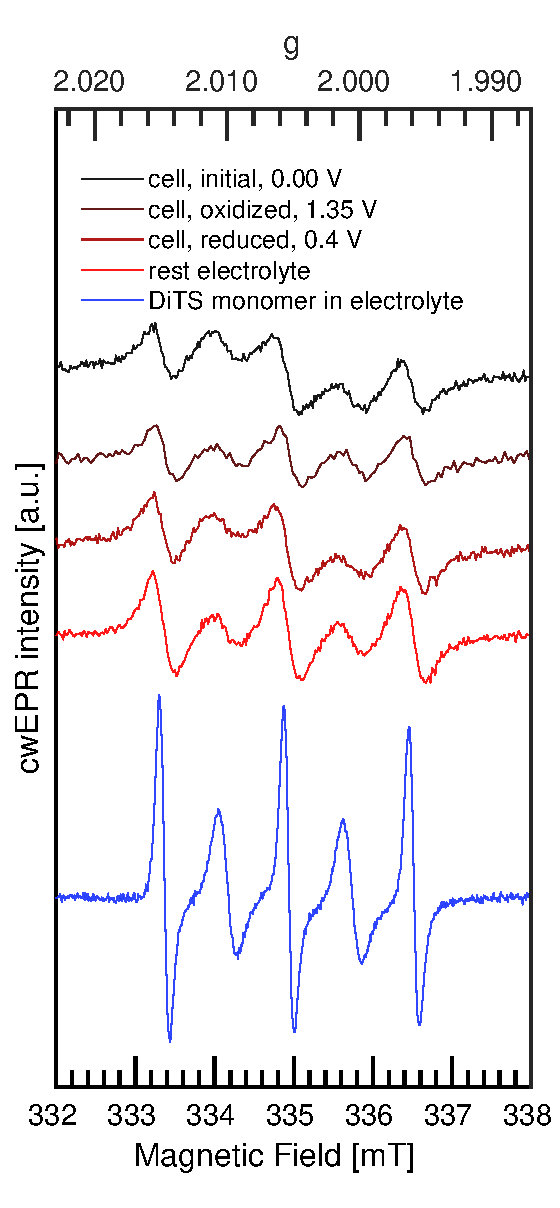
\includegraphics[width=0.40\textwidth]{./operando_epr/figures/Figure_S5}
\caption{Top: Room temperature SEC cwEPR on 150-CV p-DiTS film. $\nu=$~9.4~GHz. This film has not undergone the cleaning/rinsing procedure and therefore as expected we see spectral signatures of the DiTS monomer which is released into the electrolyte and exhibits a five-line structure characteristic of di-TEMPO systems with changes in the exchange coupling associated with changes in the nitroxide -- nitroxide distance. This figure shows the primary release of monomeric DiTS from a raw p-DiTS film into electrolyte (Modulation amplitude 0.1~mT -- overmodulated). Bottom: cwEPR of DiTS monomer in electrolyte 100~$\muup$\textsc{m} concentration at room temperature for comparison (Modulation amplitude 0.02~mT).}
\label{fig:S5}
\end{figure}
Fig.~\ref{fig:S5} shows the in-operando study on a 150-deposition-cycle $t =$~400~nm film, that has not undergone the cleaning procedure. Here the non-polymerized monomeric DiTS is released into electrolyte, confirmed by measuring the in-operando and used electrolyte cwEPR spectra, along with comparison to a 100~$\muup$\textsc{m} sample of monomeric DiTS in solution.
\newpage
\begin{figure}[H]
\center
	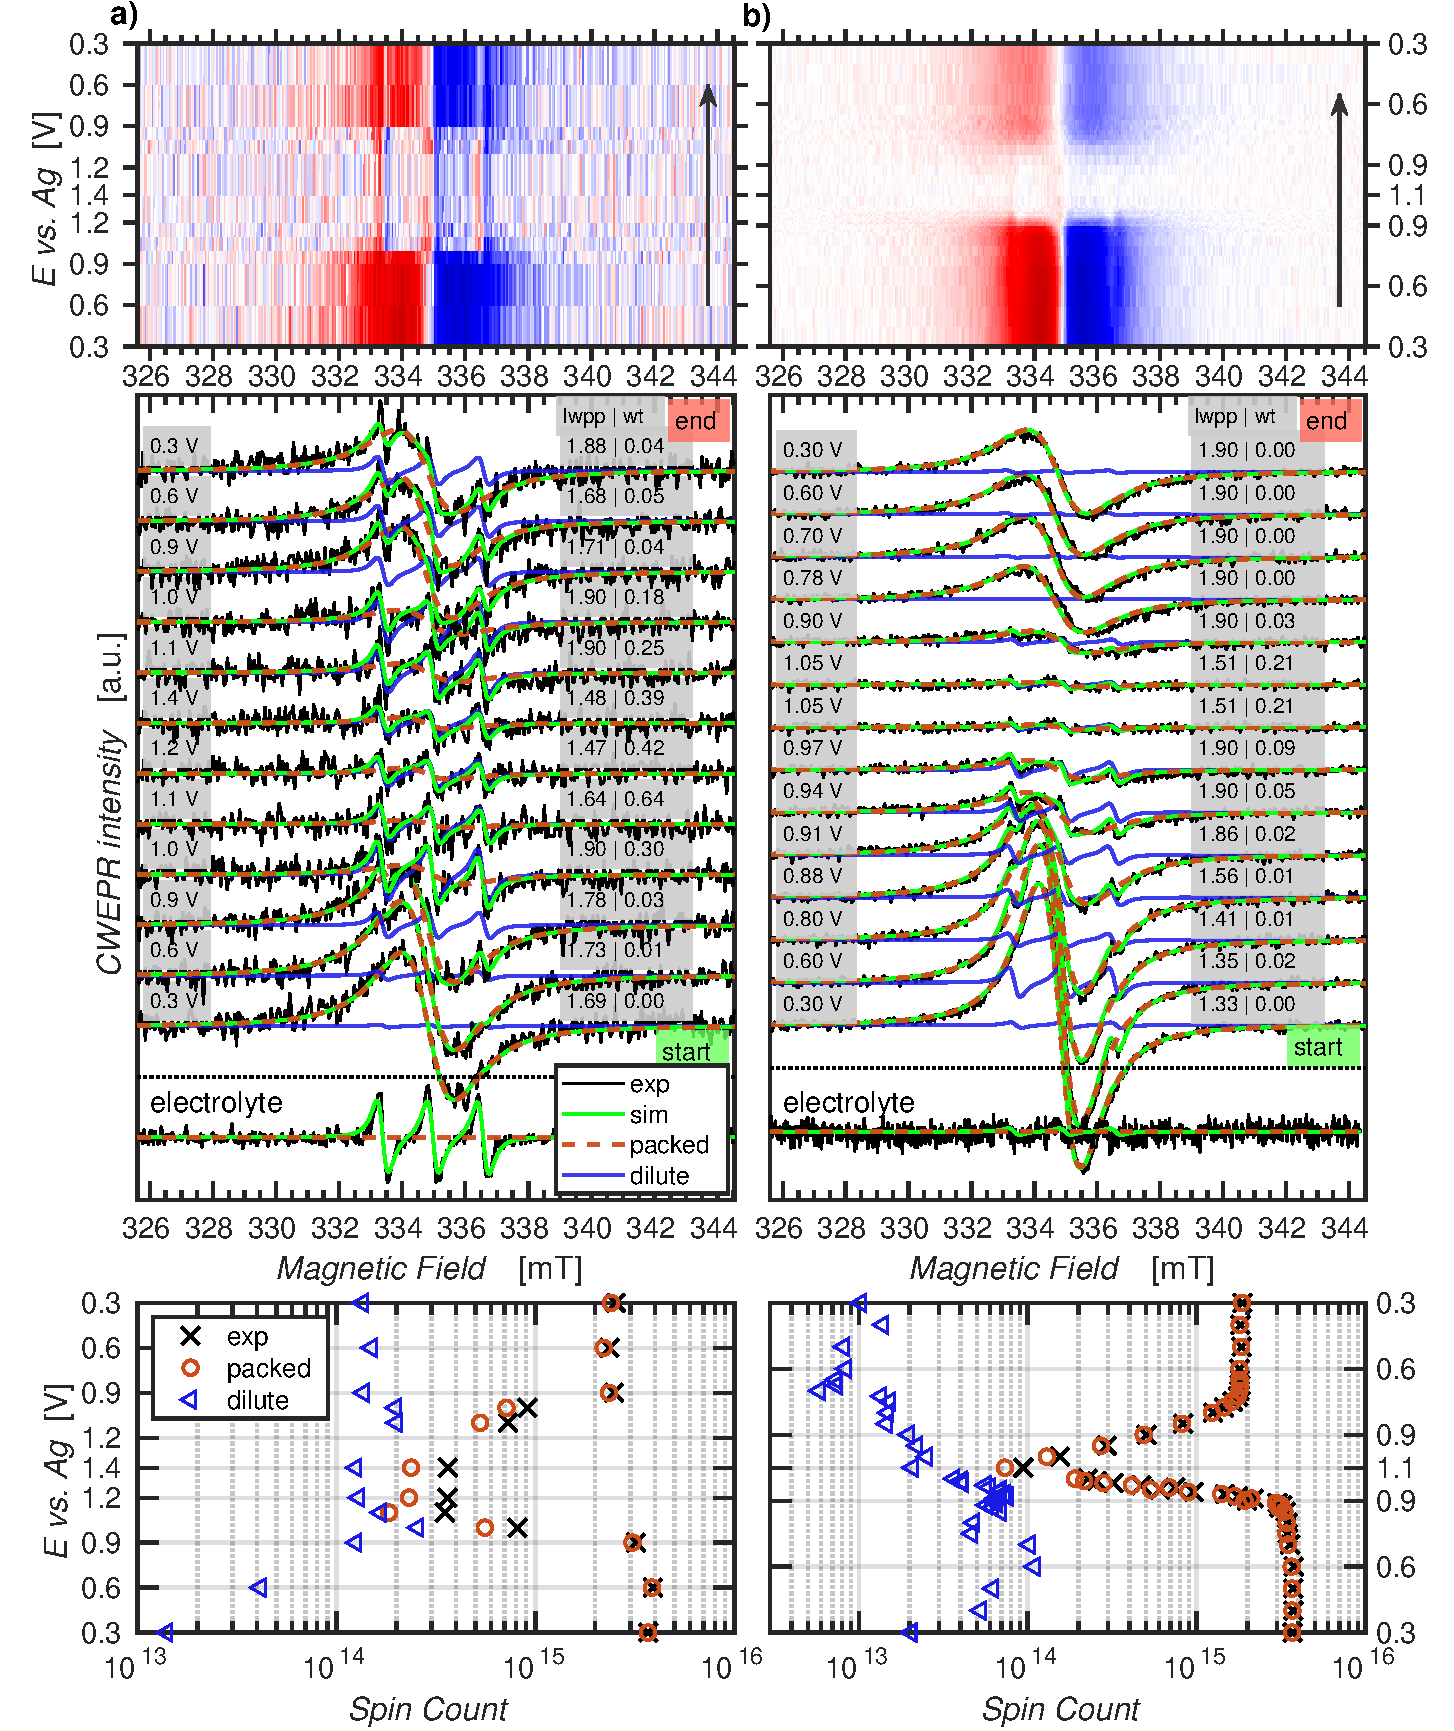
\includegraphics[width=1\textwidth]{./operando_epr/figures/degradation/operando_degradation_dits.pdf}
\caption{Room-temperature in-operando cwEPR measurements for two p-DiTS electrochemical cells. $\nu=$9.4~GHz. Two-component spectral deconvolution to identify dilute and packed nitroxide fragments. Spectrum of the rest electrolyte. a): Cell with a p-DiTS film grown by 150 deposition cycles ($t\approx 400$~nm) that was left untreated and underwent one charge-discharge cycle before the measurement. The dilute component is released during the oxidation and remains detectable in the rest electrolyte. b): Cell with a p-DiTS film grown by 200 deposition cycles ($t\approx 500$~nm) that was rinsed in solvents and cycled in the electrolyte to remove the not polymerized nitroxide fragments. The initially released dilute component is electrochemically active and does not appear in the rest electrolyte.}
\label{fig:S6}
\end{figure}


Fig.~\ref{fig:S6} shows more steps in the in-operando study shown in Fig.~\ref{fig:Figure_5}






\subsection{Spectral Simulations}
The cwEPR spectra for a pDiTS film in Figure~\ref{fig:operando_carpet} consist of a combination of the characteristic signals specified in Figure~\ref{fig:cartoon_spectra_dts}. In order to separate the spectral contribution and to perform a quantitative analysis of the separated components, a numerical simulation of the spectra was performed.


\subsection{Quantitative Analysis of Potential-Dependent EPR Spectra}
\label{sec:quantitative_EPR}
\begin{figure}[h]
\center
	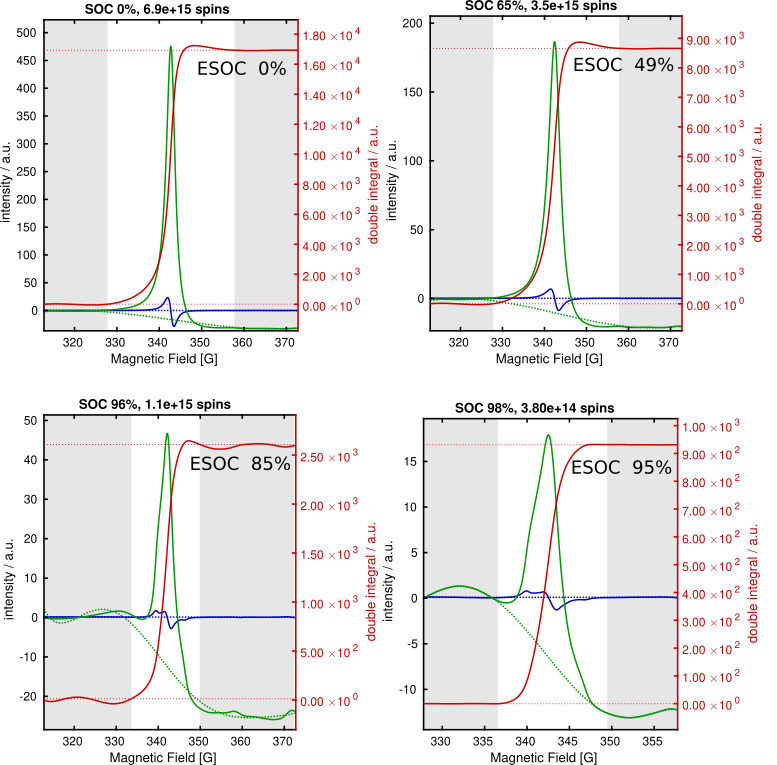
\includegraphics[width=0.85\textwidth]{./pulse/figures/Figure_S6}
	\caption{cwEPR spectra for a pDiTBuS film in four charge states. Single and double integrals of the signal. Spin count is proportional to the end value of the double integral. Temperature: 80~K, $\nu\approx$~9.6~GHz, field modulation: 5~G at 100~kHz. ER~4118 X-MD5 dielectric ring resonator.}
	\label{fig:Figure_S6}
\end{figure}

The number of spins at each SoC was determined with quantitative cwEPR from the double integral of the cwEPR intensity calculated with the Spincounting Toolbox~\cite{spin_counting_tb} for Matlab~\cite{SI:Matlab}. The cwEPR spectra in Figure~\ref{fig:Figure_S6} were measured in a Bruker Elexsys E580 spectrometer equipped with an ER 4118 X-MD5 dielectric ring resonator with an unknown Q factor. To calibrate the intensity of the measured cwEPR signals and to determine the absolute number of spins in the film, we measured the cwEPR spectrum of the fully discharged film (SoC 0\%) with a calibrated spectrometer. The calibrated spectrometer is a lab-built X-band cwEPR spectrometer equipped with a 9.4~GHz, 200~mW microwave source and a 4122-SHQE resonator. With Q~$=6095$, the absolute number of spins in the pDiTBuS film at SoC~0\% was measured to be $N=(6.9\pm0.4)\times10^{15}$. We used $N$ to get the number of spins for other SoC from the spectra measured with the uncalibrated spectrometer. We assumed that the Q factor of the resonator remains the same for different SoC~\cite{Kulikov2022} and computed the corresponding numbers of spins from the doubly integrated spectral intensities.\\

The doubly integrated cwEPR spectral intensities for the pDiTBuS film in the four considered SoC relate to each other as 100:51:15:6 with the absolute number of spins of $(6.9\pm0.4)\times10^{15}$, $(3.5\pm0.2)\times10^{15}$, $(1.1\pm0.1)\times10^{15}$ and $(3.8\pm0.4)\times10^{14}$, respectively. The respective ESOC are therefore $(0\pm5)$\%, $(49\pm3)$\%, $(85\pm2)$\% and $(95\pm1)$\%. Spin \rs{concentrations} in the film are $(5.3\pm2.7)\times10^{20}$, $(2.7\pm1.4)\times10^{20}$, $(0.8\pm0.4)\times10^{20}$ and $(0.3\pm0.2)\times10^{20}$ cm$^{-3}$, respectively. Integration of the cyclic voltammogram yields $(2.3\pm0.8)\times10^{16}$ electrons in the reduced state.\\
%The relative intensities of the CWEPR signals correspond to ESOC 0\%, 49\%, 85\% and 95\%.
%\newpage



\subsection{Spectra of NiSalen Films}
The molecular backbone of pDiTS and pDiTBuS is the pNiSalen, a conjugated polymer that exhibits redox behavior~\cite{Dmitrieva2018,Vereshchagin2020,Apraksin2021}. The observations of electrochromicity of pNiSalen films with UV-VIS spectroscopy~\cite{Dmitrieva2018} have revealed the formation of polarons and antiferromagnetically coupled (with total spin S=0) bipolarons in the oxidized state of pNiSalen. A series of cwEPR spectra recorded for a pNiSalen film in various redox states is shown in Figure~\ref{fig:cwEPR_CRYO_NiSalen_REDOX_SIM}. Operando cwEPR spectra of a cell containing a pNiSalen cathode is shown in Figure~\ref{fig:cwEPR_RT_NiSalen_OPERANDO}. Remarkably, there was no signature of pNiSalen observed in TEMPO-Salen cells shown in Section~\ref{sec:operando_dits}.

\begin{figure}[!h]
\center
	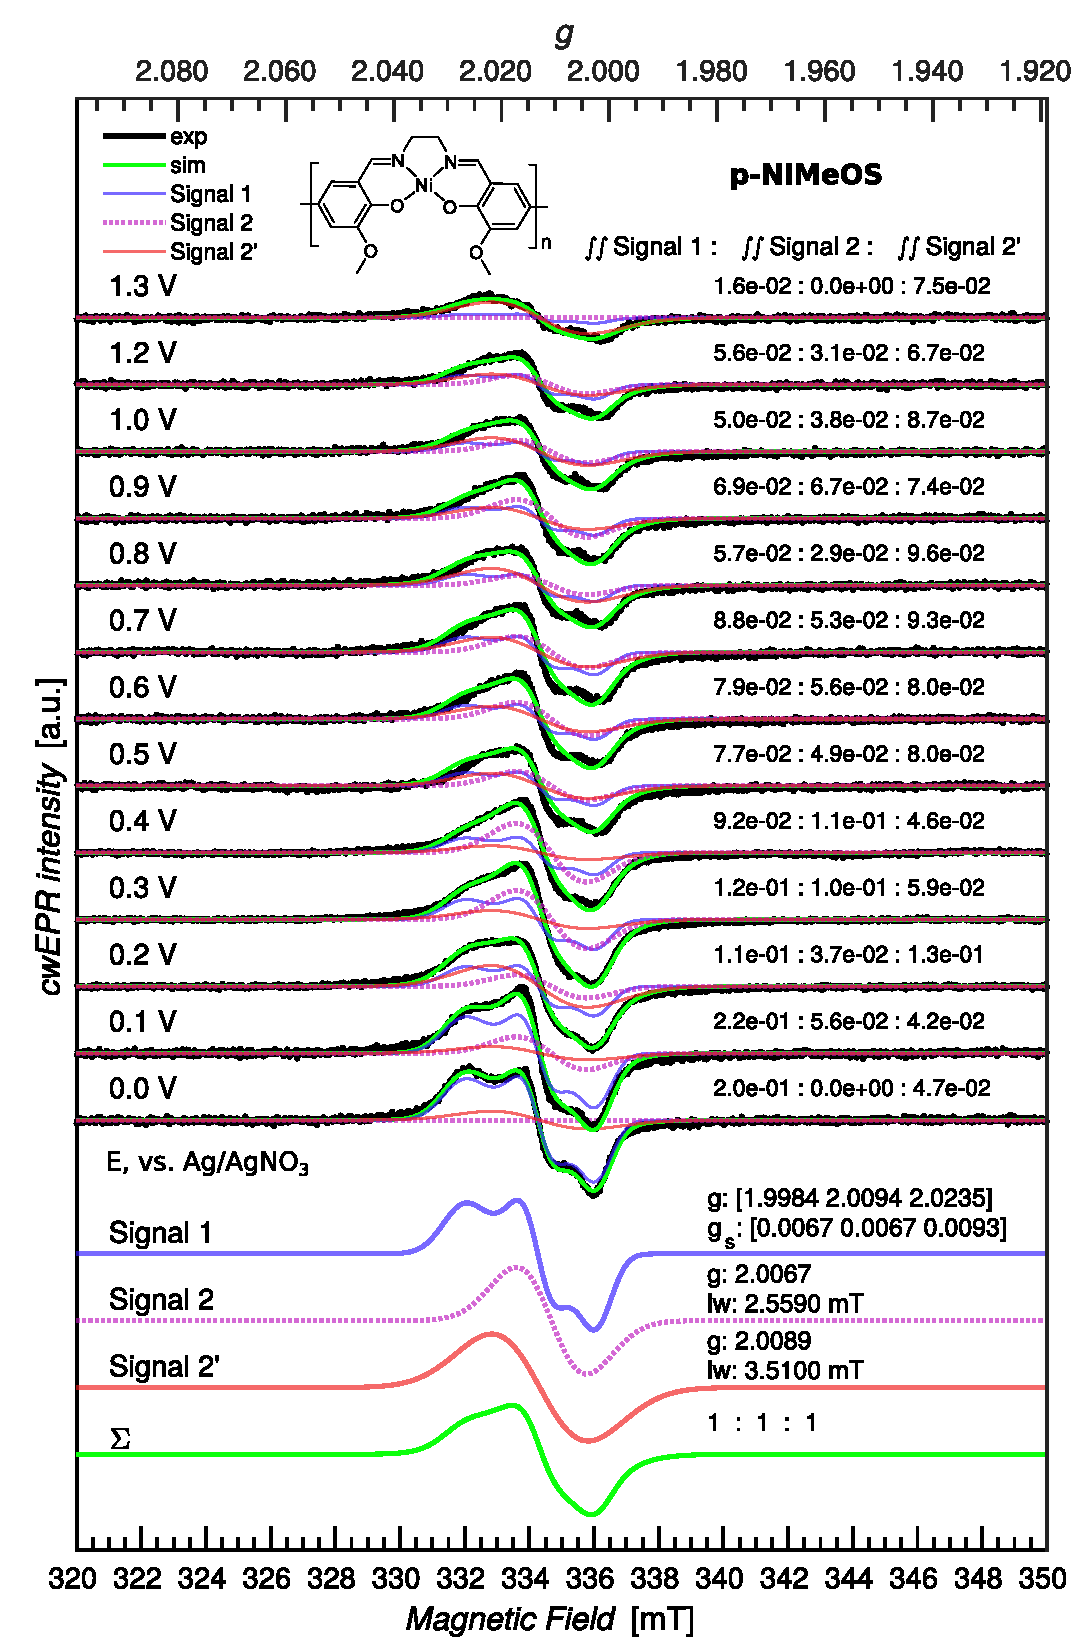
\includegraphics[width=0.9\textwidth]{./operando_epr/figures/CRYO/Figure_S8.pdf}
	\caption{Potential-dependent cwEPR spectra of a NiMeOSalen film measured at 150~K. Simulation of the spectra with three components reported by the Timonov group.}
	\label{fig:cwEPR_CRYO_NiSalen_REDOX_SIM}
\end{figure}

\begin{figure}[!ht]
\center
	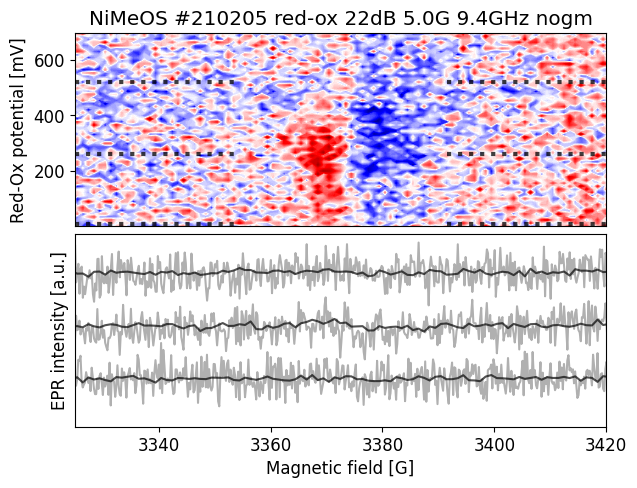
\includegraphics[width=0.8\textwidth]{./operando_epr/figures/backbone/NiMeOS_lyra_overnight_RT.png}
	\caption{Potential-dependent operando cwEPR spectra of a NiMeOSalen cathode film measured at room temperature.}
	\label{fig:cwEPR_RT_NiSalen_OPERANDO}
\end{figure}

\section{Monitoring of Degradation Processes}
\label{Degradation_study}
The operando monitoring of EPR spectra in pDiTS cells has revealed that the amount of paramagnetic species reduces upon the cycling. The cwEPR spectra during one charge-discharge cycle of two different pDiTS cells are shown in Figure~\ref{fig:operando_degradation}. Both datasets show a significant amount of the three-line structure in the oxidised (fully charged) state, that corresponds to the the release of dilute nitroxide radicals from the polymer film to the electrolyte. The fact that the released species exhibit a 3-line structure and not a 5-line structure excludes the release of the di-TEMPO (DiTS) monomers and suggests that individual TEMPO$^{\bullet}$ fragments are being detached from the film. Therefore, it was found that it is the molecular degradation of DiTS that is responsible for the loss of cell's capacity and not the decomposition of the polymer film into the monomer fragments. The overall EPR signal intensity decreases for both samples after the charge-discharge cycle. The spectral deconvolution with quantitative analysis of the individual components has revealed that the released fragments do not explain the overall loss of the signal intensity after the cycle.\\


\begin{figure}[!h]
\center
	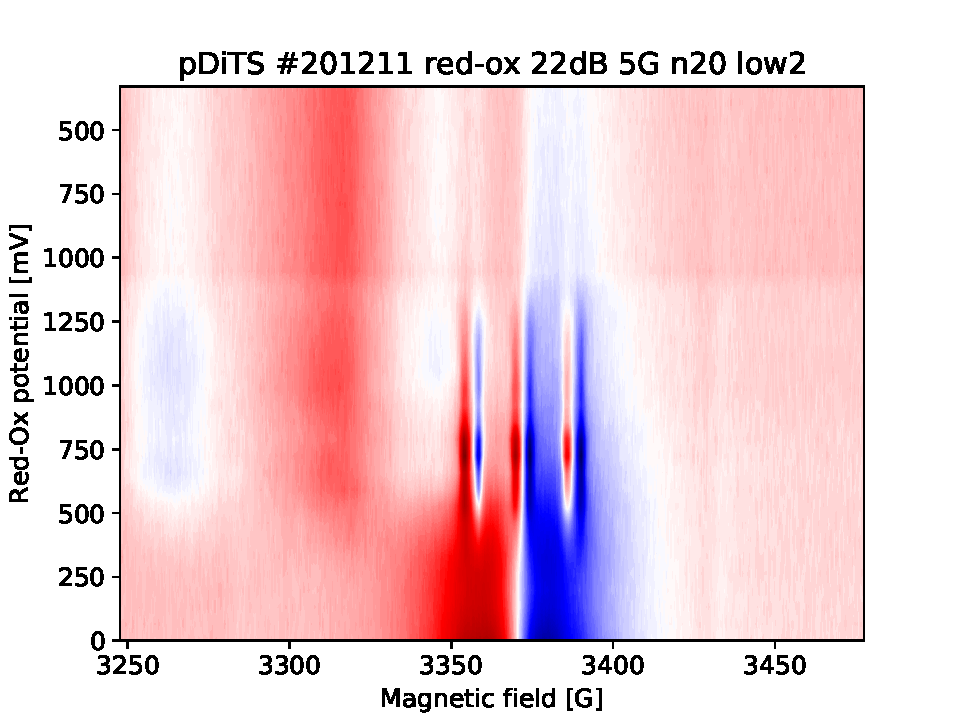
\includegraphics[width=1\textwidth]{./operando_epr/figures/degradation/overnight_dits_201211_full_redox_contour_XY.pdf}
	\caption{Operando cwEPR spectra of a pDiTS electrochemical cell showing irreversible release of charge-bearing fragments and decomposition of the device upon potentiostatic charging with currents up to $I<0.2$~mA~$\approx125$~C.}
	\label{fig:operando_degradation_device}
\end{figure}


\begin{figure}[!h]
\center
	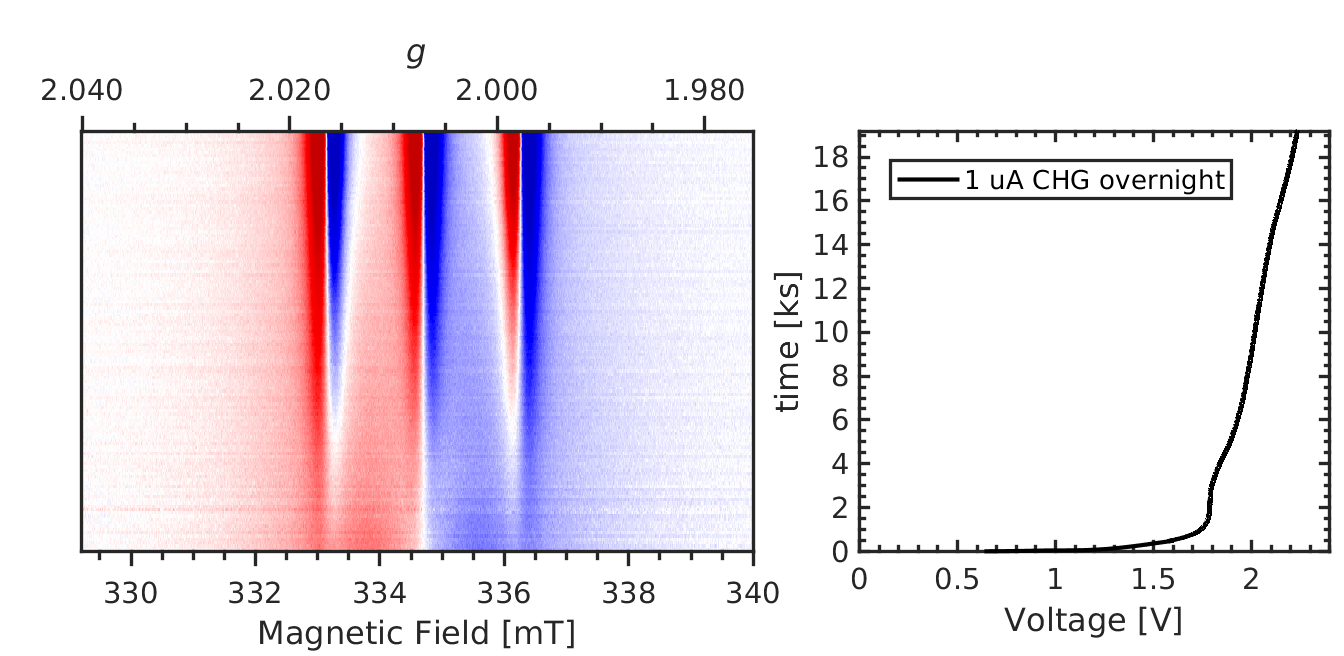
\includegraphics[width=1\textwidth]{./operando_epr/figures/degradation/pDiTS_slow_charge_MS5000_forslides.png}
	\caption{Operando cwEPR spectra of a pDiTS electrochemical cell showing irreversible release of charge-bearing fragments upon moderate charging currents.}
	\label{fig:operando_degradation_3_lines_release}
\end{figure}



\par
ORBs based on p-DiTS were shown to lose their capacity under repeated charge-discharge cycling,\cite{vereshchagin2020} but the mechanism of degradation is not yet understood on the molecular level. In order to study the processes occurring during degradation, we recorded CV curves along with cwEPR spectra during charge-discharge cycling of a tube-based p-DiTS electrochemical cell.

\par
For this purpose, a 400$\pm$50~nm thick p-DiTS film (Fig.~\ref{fig:S3}d, ESI$\dag$) was deposited onto the on-substrate WE. The cell was inserted into the microwave resonator of the cwEPR spectrometer at $H$ $\approx$~12~mm where it underwent a series of 36 charge-discharge cycles at a rate of 5~mV\,s\textsuperscript{-1}. The CV curves were recorded for each cycle. The cwEPR spectra were recorded after each fourth cycle for the fully reduced/discharged cell, that is at the left-most point on the corresponding CV.

\par
Fig.~\ref{fig:Figure_6} shows the cwEPR spectra (a) and the CV curves (c) measured during the repeated cycling of the electrochemical cell. During the cycling, the CV curves decrease in intensity, indicating a decrease in the number of the electrochemically active charges in the film. The number of electrochemically active charges was determined for each cycle by integrating the reduction branch of the corresponding CV. It is plotted together with the quantitative EPR results, labeled as ``CV'' in Fig.~\ref{fig:Figure_6}b. The spectra, CV and quantitative analysis for the intermediate cycles are shown in Fig.~\ref{fig:S9} (ESI$\dag$).

\par
The cwEPR spectra in Fig.~\ref{fig:Figure_6}a demonstrate an initial release of the dilute component and a decrease in intensity upon further cycling. The three-line dilute component corresponds to TEMPO$^{\bullet}$ fragments that detach from the film in the reduced state and get released to the electrolyte. The dilute component is emerging only during the first eight cycles. Meanwhile, the amplitude of the CV (cf.\ Fig.~\ref{fig:Figure_6}c) stays as high as 100~$\muup$A during the first eight cycles. This suggests that the initial release of the reduced, EPR-active TEMPO fragments does not significantly affect the capacity of the cell and can be excluded as the main degradation pathway.

\par
The broad, single-line packed component, on the contrary, keeps decreasing for $>$8 cycles, together with the CV. Therefore, the degradation of the electrical capacity of the p-DiTS film has to be associated with the decrease in the signal intensity of the packed component and is not accompanied by the release of any EPR-active products to the electrolyte.

\par
The number of paramagnetic states in the film after each degradation step, as determined by a quantitative analysis of the respective spectral components, is shown in Fig.~\ref{fig:Figure_6}b along with the number of electrically active charge carriers. For the fresh film (``0~CV''), the quantitative EPR and CV results are in good agreement. In contrast, there is a significant difference after 36 cycles. This experimental observation can be rationalized as follows.

\par
All cwEPR spectra in Fig.~\ref{fig:Figure_6}a were recorded when the film was brought to the reduced state, with all electrochemically active TEMPO$^\bullet$ fragments being also EPR active. Additionally, all electrochemically inactive fragments that happen to be in the reduced, TEMPO$^\bullet$ state also contribute to the cwEPR signal. Thus, the cwEPR signal after each charge-discharge cycle contains contributions from \emph{electrochemically active} and \emph{electrochemically inactive} TEMPO$^\bullet$ fragments, and both components contribute to the overall number of spins shown in Fig.~\ref{fig:Figure_6}b.

\par
The intensity of the packed spectral component substantially decreases with cycling. This indicates that some paramagnetic parts of the film (TEMPO$^{\bullet}$) become diamagnetic (TEMPO$^{+}$) and stay EPR silent when the cell is brought back to the reduced state. These fragments may either stay in the film or to be released into the electrolyte. 
As a previous study reported no loss of mass of a p-DiTS film in a microbalance-monitored charge-discarge cycling, \cite{vereshchagin2020} we assume that the oxidized and electrically disconnected, EPR silent fragments do not leave the film.



\par
Upon cycling, the number of electrochemically active charged species decreases stronger than the number of paramagnetic states (Fig.~\ref{fig:Figure_6}b). This  indicates that some regions of the film become redox inactive upon cycling but still contribute to the EPR spectrum. These TEMPO$^{\bullet}$ fragments lose the electrical connection to the rest of the film (and thus to the metal electrode) and stay in the reduced state. The possible degradation of a p-DiTS film leads to the interruption of a conductivity pathway, resulting in the formation of electrically isolated domains within the film. We suggest that these isolated domains are also responsible for the remaining packed EPR signals observed for the nominally fully-oxidized film in the in-operando redox measurement (Fig.~\ref{fig:Figure_4}).


\begin{figure}[!h]
\center
	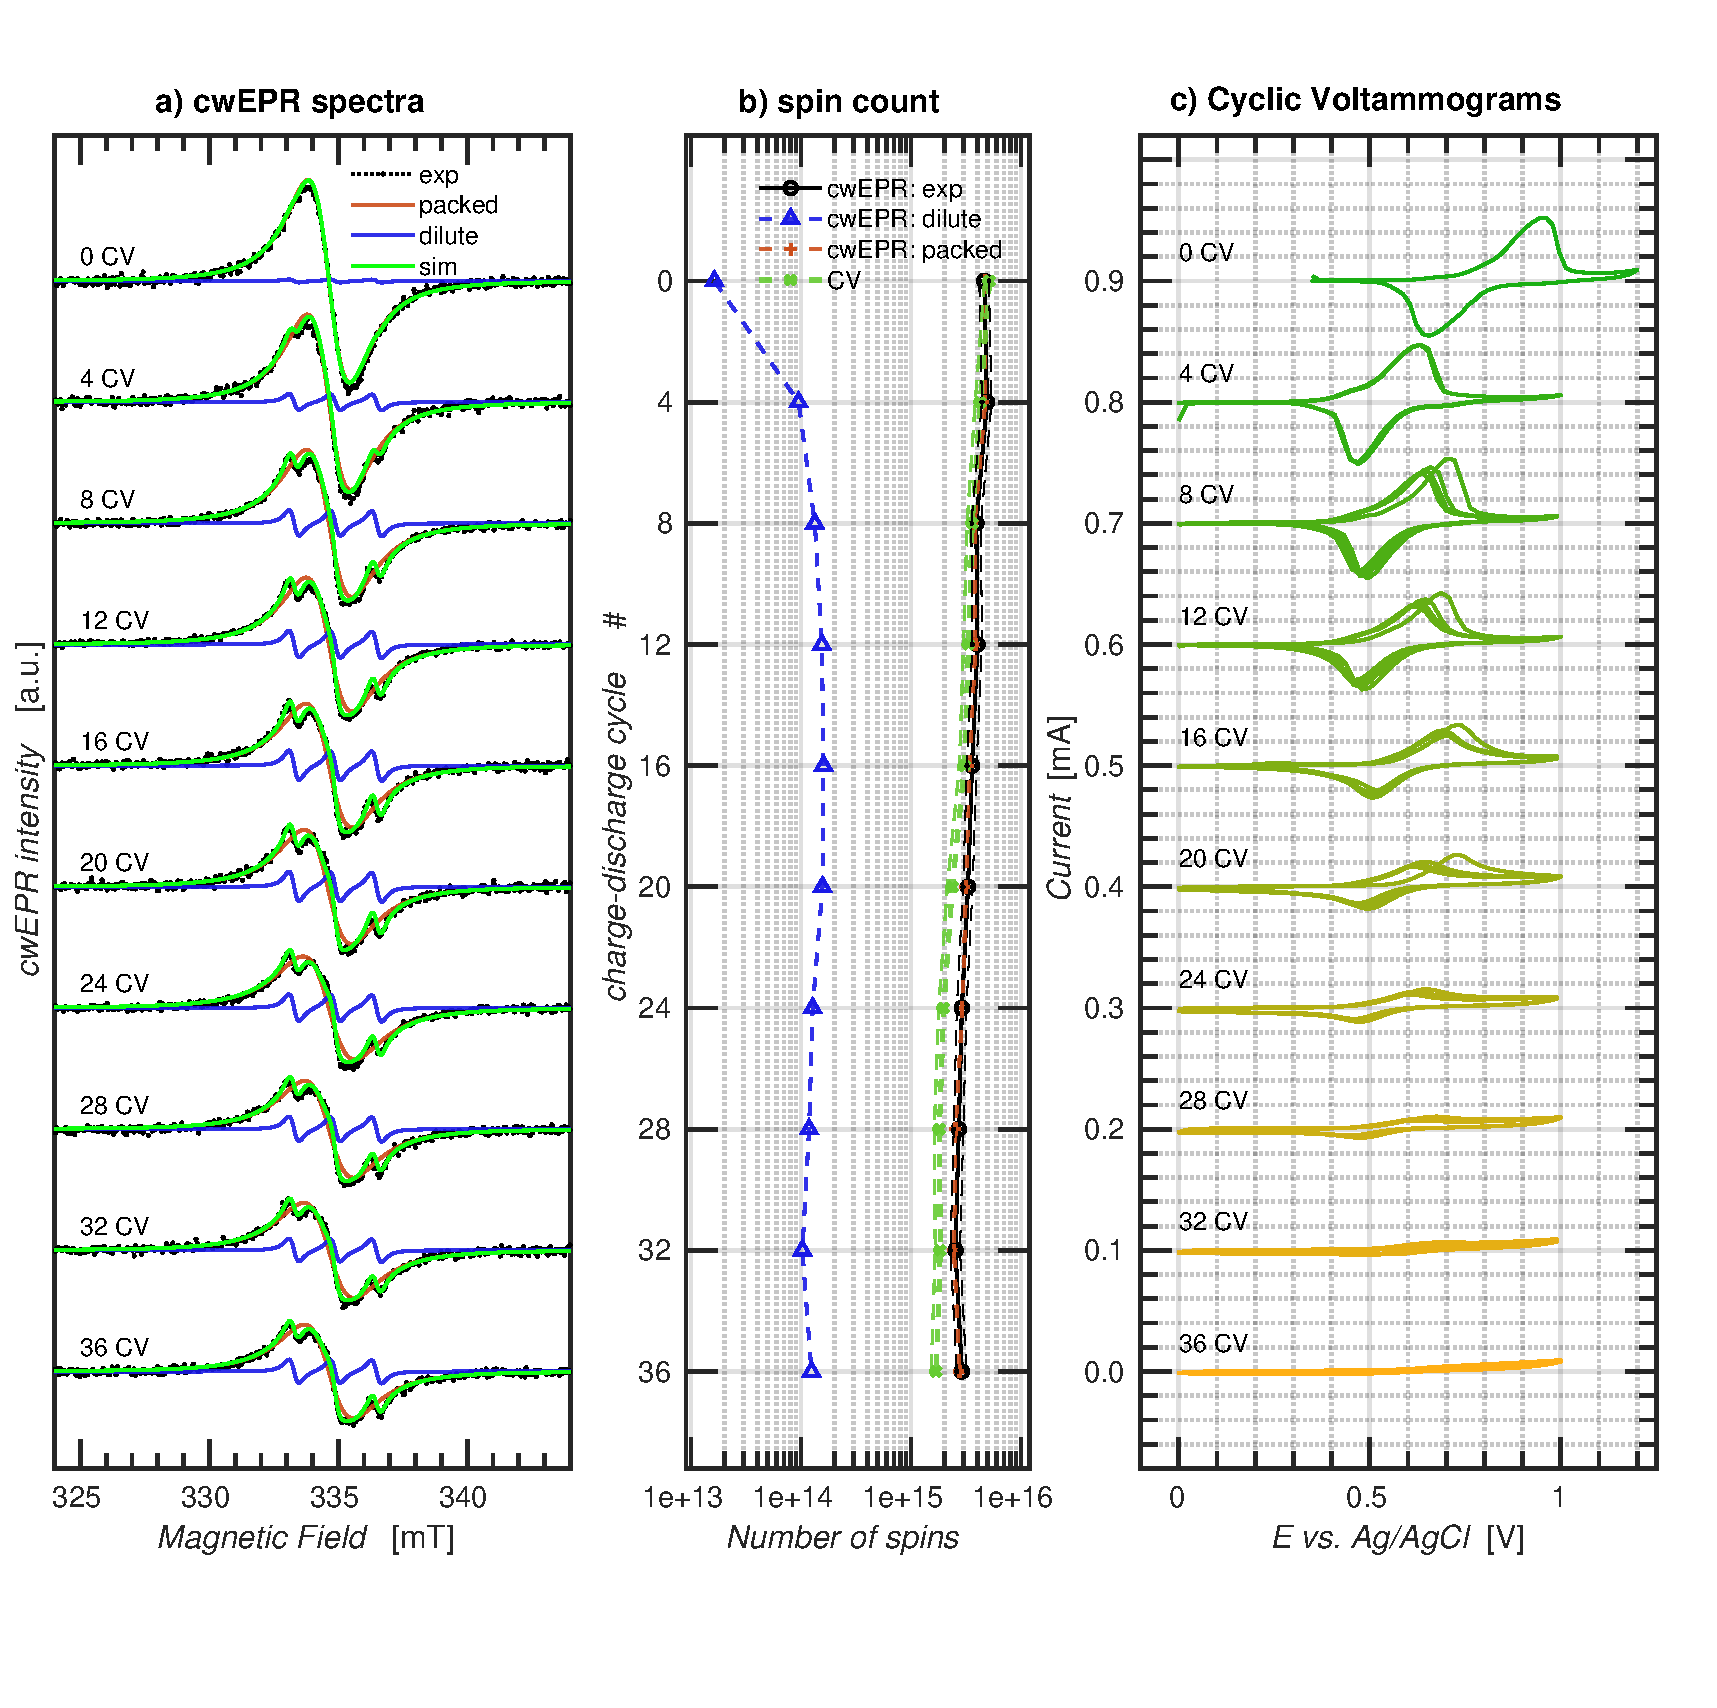
\includegraphics[width=1\textwidth]{./operando_epr/figures/degradation/repeated_cycling_degradation_dits.pdf}
	\caption{a): Evolution and component decomposition of cwEPR spectra for a tube-based, 150~CV p-DiTS ORB upon 36 charge-discharge cycles. b): Quantitative analysis of the separated spectral components. $\nu$ = 9.4$\,$GHz, Mod.~Amp:~0.5$\,$mT. Quantitative analysis of the CV curves. c): Cyclic voltammograms of the cell, recorded with respect to Ag/AgCl RE at a rate of 5~mV\,s\textsuperscript{-1} in between the EPR scans, in the modified tube inside the microwave resonator. The CV were taken at 5~mV\,s\textsuperscript{-1}, which is 10 times slower than the CV curves taken in the larger beaker, because limited amount of the electrolyte in the modified tube was found to strongly affect the shape and positions of the CV peaks at higher speeds of cycling.}
	\label{fig:repeated_cycling_degradation}
\end{figure}


\begin{figure*}[ht!]
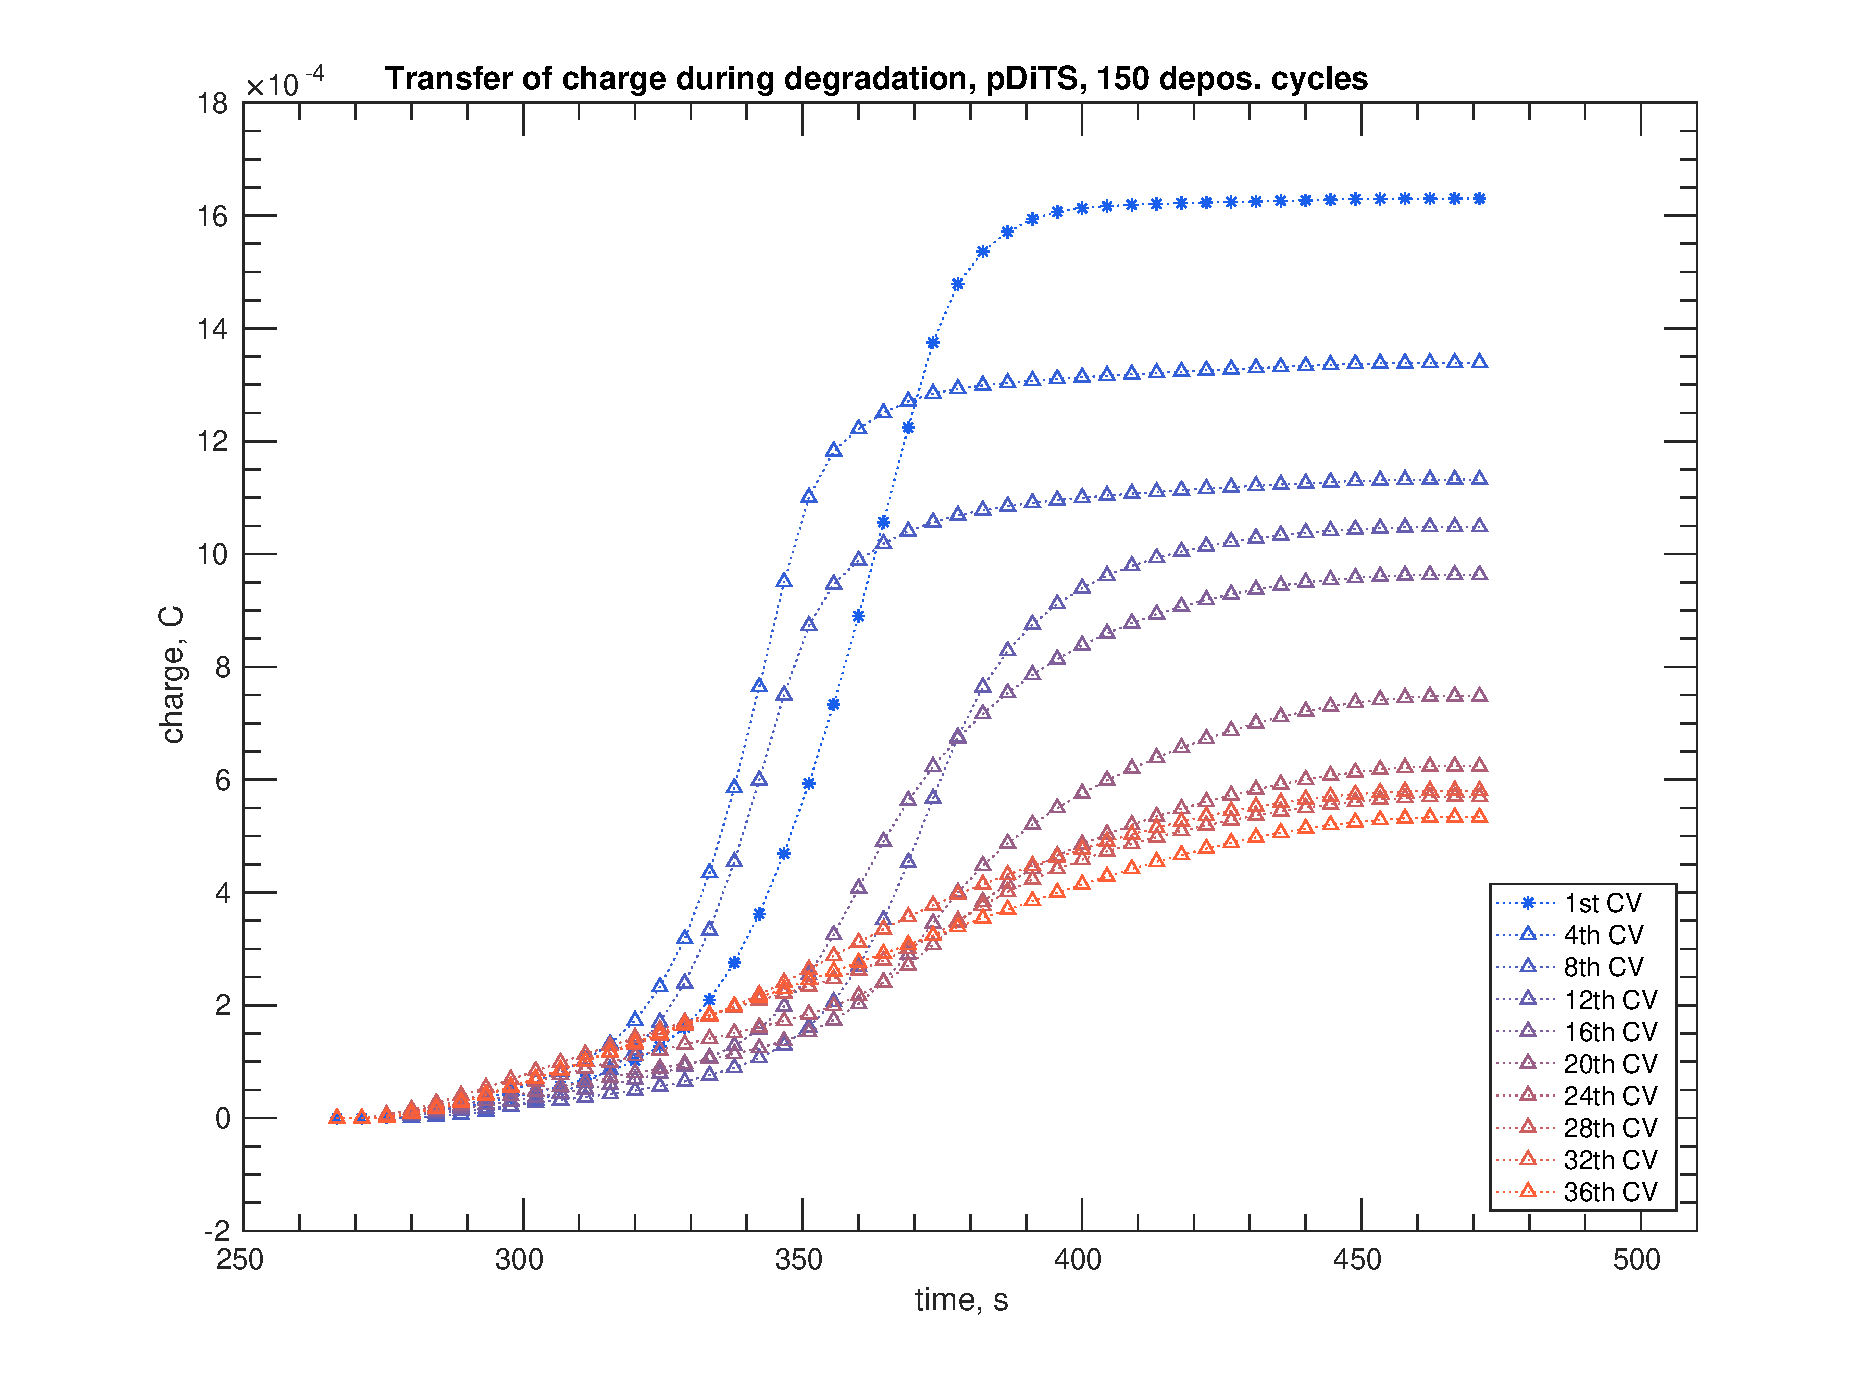
\includegraphics[width=0.9\textwidth]{./operando_epr/figures/degradation/Figure_S10}
\caption{Degradation of capacity of a p-DiTS film upon 36 charge-discharge cycles. Transferred charge calculated as integrals of the reduction branches of the CV curves. By the last charge-discharge cycle the film can accept 10 times less the charge as in the beginning of the cycling.}
\label{fig:S10}
\end{figure*}


The degradation of p-DiTS cells was monitored simultaneously by cwEPR and cyclic voltammetry. The number of paramagnetic species in the cells was changing during the degradation cycling. That change was quantified from both EPR and electro-chemistry perspective. Quantitative analysis of the simulated components comprising the cwEPR spectra was done with the Spincounting Toolbox\cite{spin_counting_tb} (developed by Christopher Engelhard) in Matlab. Cells with the electrolyte exhibit weaker signals as compared to the dry films, so an intensity scaling factor was determined and taken into account.

\bigbreak

The CV curves during the degradation of the cells were quantitatevly analyzed. The reduction branches were integrated versus time to obtain the charge transferred to the film at each degradation cycle. The integrals are shown in \ref{fig:S10}. The total transferred charge during the reduction of the film is a three-electron process,\cite{si_vereshchagin2020} where two electrons are transferred to the TEMPO groups and one electron is transferred to the backbone. Therefore, the number of electrons transferred to TEMPO is $2/3$ of the total charge transferred to the film divided by the elementary charge. With that, the number of electro-chemically active TEMPO groups was determined at each degradation cycle.

\bigbreak

We observed two pathways of the degradation of p-DiTS: the release of paramagnetic nitroxide fragments and the overall decrease in the cwEPR signal after a charge-discharge cycle, that is connected to the formation of diamagnetic, or oxidized, electrically isolated domains within the film. The latter may, possibly, be accompanied by a release of the diamagnetic fragments to the electrolyte.

\bigbreak

While the cell in \ref{fig:S6}~a almost fully recovers its initial signal intensity, the cell in Fig.~\ref{fig:S6}~b loses 51$\%$ of its initial spin count after being reduced back to its paramagnetic state (from 8.0E+15 spins to 3.7E+15 spins, cf. Fig.~\ref{fig:S6}, bottom subplots for the spin count data). That indicates, some fragments have lost electrical connection to the rest of the film, and stayed in an oxidized, diamagnetic state. The dramatic decrease in spin count can be accounted for by the disappearing "dilute" component only partially, as the dilute component yields maximum 2.7E+14 spins (at 600~mV) which is only 3$\%$ of the total spin count. The remaining 48$\%$ of missing spins can not be explained by the release of paramagnetic fragments. We propose that some fragments of the film are losing connection to the film during the oxidation process. These EPR silent, oxidized nitroxide fragments may stay in the film or may leave it. That process is observed only indirectly as a change of the overall EPR signal intensity, when the cell undergoes a full charge-discharge cycle.



\section{Monitoring of Self Discharge}
Organic Radical Batteries have a tendency to self-discharge, as the organic electrochemically active layer partially dissolves in polar electrolytes. Particularly for the TEMPO containing ORB, the dissolved, mobile TEMPO fragments serve as redox shuttles that carry the charge between the battery electrodes and cause a self discharge. The amount of unoxidized TEMPO$^\bullet$ shuttles can be measured with cwEPR spectroscopy as the mobile fragments have distinct spectra as compared to the fragments tightly packed in the electrode. Further in this subsection operando spectra of a TEMPO containing electrochemical cells are shown. Quantitative analysis of the released fragments during a charge-discharge cycle allows for a description of the self-discharge process in an ORB. The charge state of a battery is monitored with cwEPR and, additionally, with a potentiometric measurement to identify the self-discharge rate and to connect it with the concentration of diffusing redox shuttles. Figure~\ref{fig:self_discharge_DOM} represents a gradual change in the cwEPR intensity of a self-discharging tube-based cell with a pDiTS cathode. The cell was initially discharged to $V_{OC}=350$~mV and then charged to $V_{OC}=1300$~mV, at that point the minimal cwEPR intensity was registered. The cell was left under the open circuit condition. After $t=500$~s, the cwEPR signal of the cell has fully recovered, that corresponds to the complete reduction of the electrochemically active nitroxide radicals in the cathode film.

\begin{figure}[h]
\center
	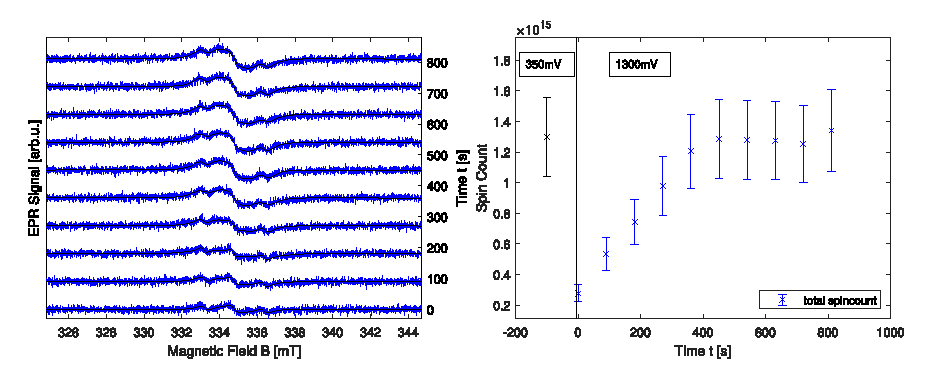
\includegraphics[width=1\textwidth]{./operando_epr/figures/self_discharge/DOM_DITS_SELF_DISCHARGE.pdf}
	\caption{cwEPR monitored self-discharge of a tube-based cell containing a pDiTS film made with 50 deposition cycles. Left: Development of the EPR spectra of the oxidised sample over time from bottom to top; Right: Development of the spincount of the oxidised sample over time and comparison to the reduced state.~\cite{DOM}}
	\label{fig:self_discharge_DOM}
\end{figure}





\begin{figure}[h]
\center
	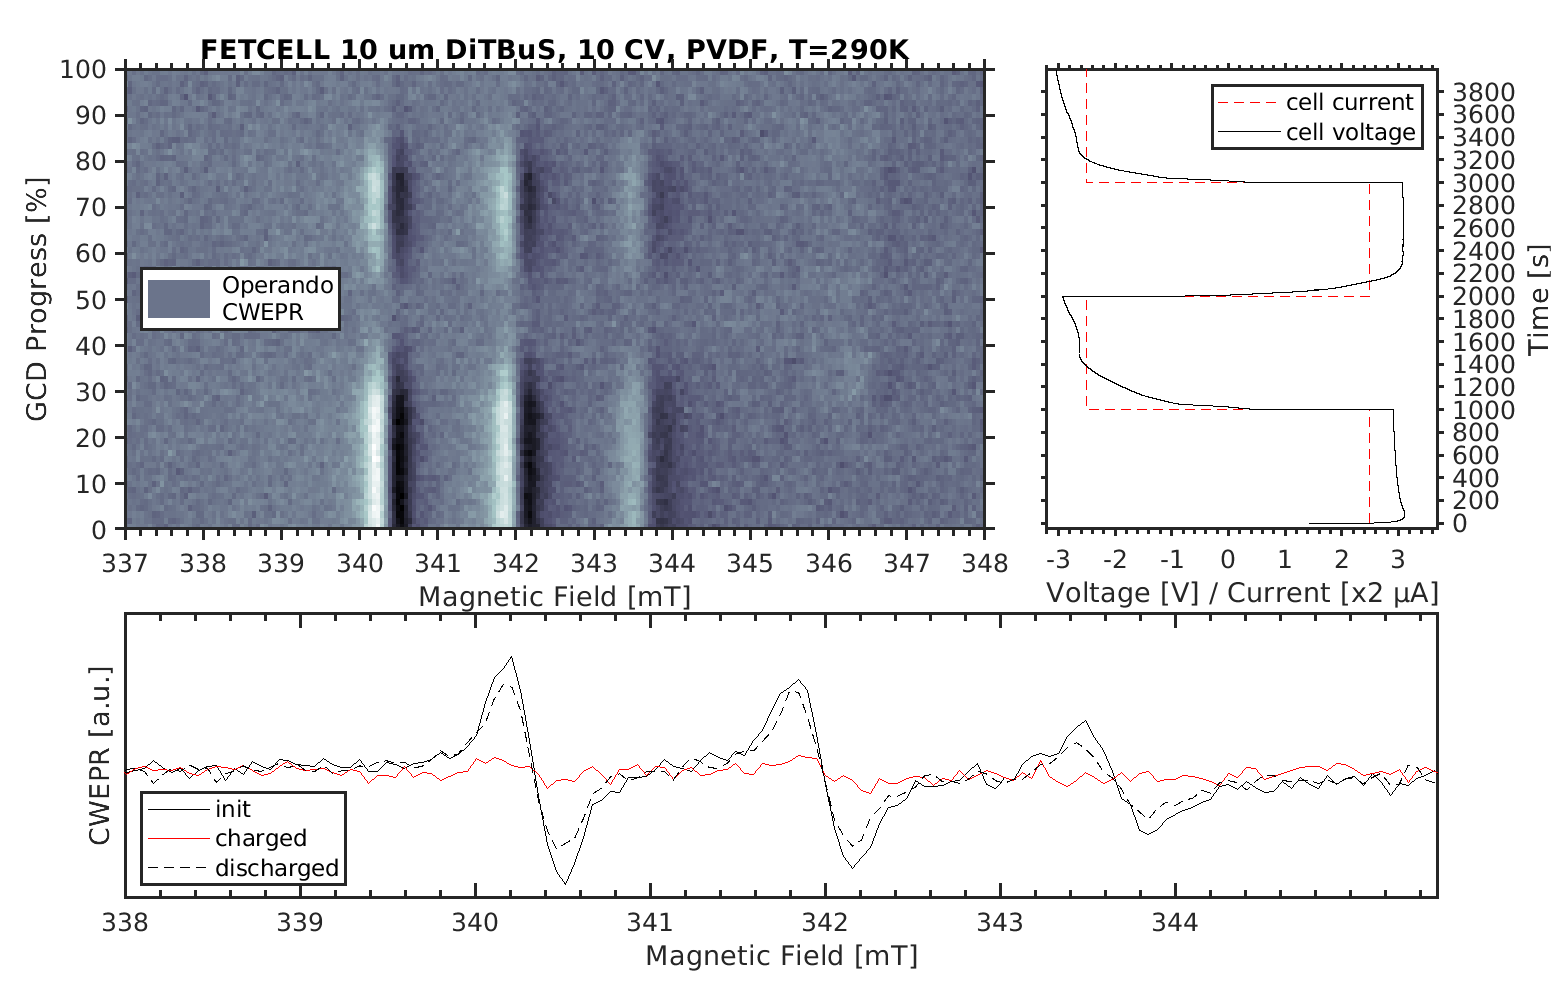
\includegraphics[width=1\textwidth]{./operando_epr/figures/solid/FET231114_5uA_RT.pdf}
	\caption{Operando cwEPR on an all-polymer organic radical battery made on a 5~$\muup$m grid with a PVDF/TFSI gel electrolyte.}
	\label{fig:operando_solid_battery}
\end{figure}

\section{Low Temperature Measurements}
\label{sec:low_T}
%
While in-operando SEC cwEPR provides information about redox systems in their natural operating environment, these measurements are limited by the time for which potentials can be applied before degradation of the active materials is observed. In contrast, in ex-situ experiments on cells without electrolyte, the desired redox states of the films can be observed for longer times without degradation effects. Additionally, ex-situ measurements can be performed at cryogenic temperatures, which drastically increases the EPR signal intensity.
%

\begin{figure*}[ht!]
\centering
	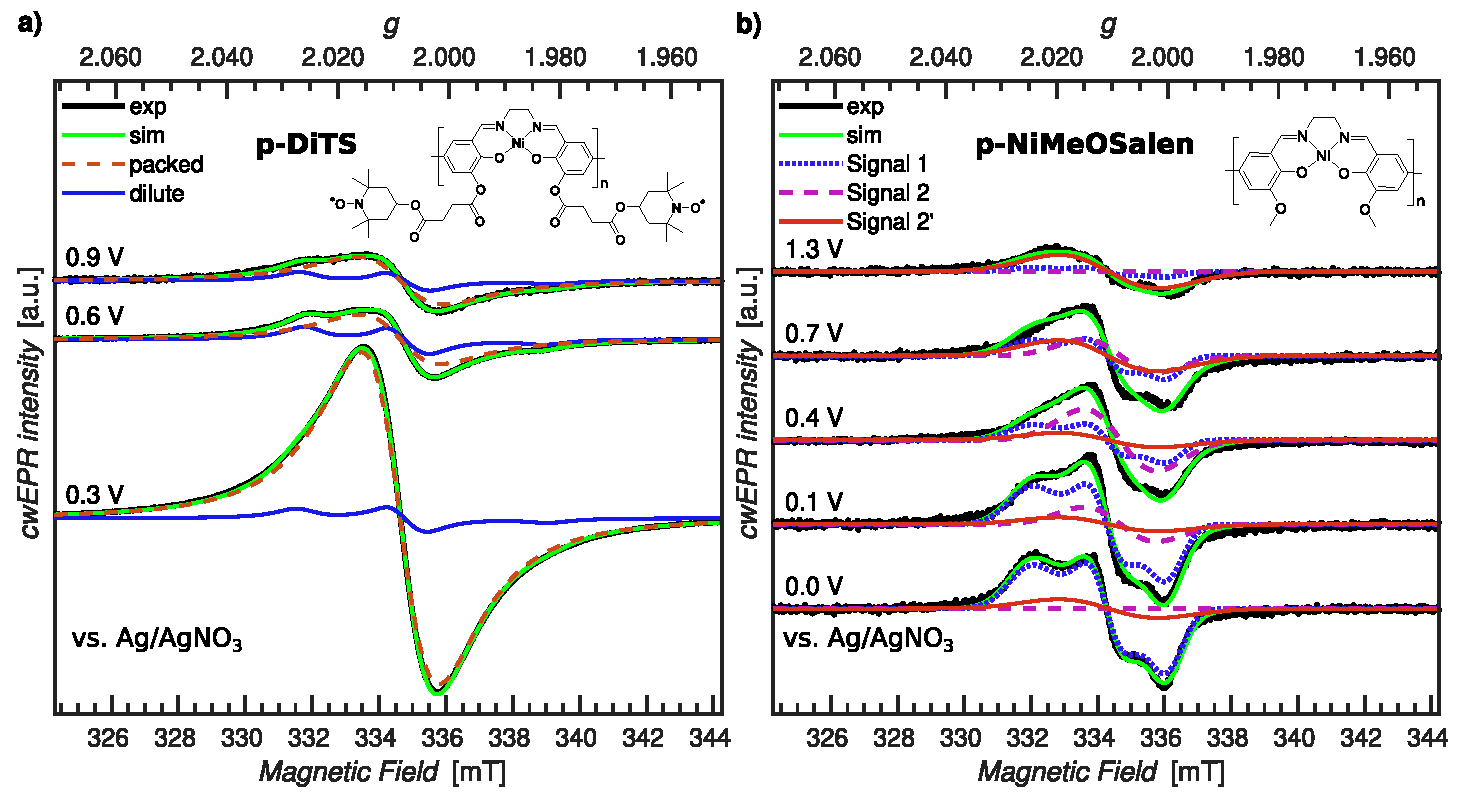
\includegraphics[width=1\textwidth]{./operando_epr/figures/CRYO/Figure_7}
	\caption{Cryogenic (150~K) ex-situ cwEPR in a range of redox potentials for p-DiTS and its molecular backbone, p-NiMeOSalen ($\nu = 9.4$~GHz). a): p-DiTS film ($t\approx400$~nm). Two-component spectral deconvolution to identify the densely packed (dashed-red curve) and dilute (solid-blue curve), immobilized nitroxide fragments. b): p-NiMeOSalen film ($t\approx900$~nm). Three-component spectral deconvolution into the components observed earlier.\cite{Dmitrieva2018}}
	\label{fig:Figure_7}
\end{figure*}


\subsection{p-DiTS} \label{Section:ex-situ_pDiTS}
%
For the p-DiTS cells, in-operando SEC cwEPR measurements were carried out at room temperature while holding the cell at redox potentials of interest for $\sim$200~seconds during the accumulation of the cwEPR spectra. The S/N for this setup is limited by the time available to acquire EPR spectra and by the low spin polarization at room temperature. We therefore perform ex-situ measurements on a 95~deposition cycle ($t =$~400$\pm$40~nm) film at cryogenic temperatures, in this case at 150~K. These ex-situ measurements involved bringing the cell to the chosen redox potential using the setup shown in Fig.~\ref{fig:Figure_1}c, outside the spectrometer. The potential was applied for 100--200~seconds. Then the electrodes were disconnected from the cell. Subsequently, the substrate with the on-substrate electrodes was placed in a standard 5~mm OD quartz tube filled with N$_2$ gas and sealed using a septum and Parafilm to prevent condensation of water in the tube. This method can hold the cell in different redox state regions but not necessarily the exact set redox potentials, as the charge seems to equilibrate to different overall states. This was determined by comparison of our ex-situ cwEPR results and spectral simulations to in-situ spectra shown in Ref.~\cite{Dmitrieva2018}. The aim of the ex-situ measurement was to reach representative redox states which were also seen in the in-operando measurements (Fig.~\ref{fig:Figure_4}), i.e. fully reduced, partially oxidized and fully oxidized states, with a higher S/N.


\par
We therefore measure the ex-situ SEC cwEPR at different oxidation potentials, three of which are shown in Fig.~\ref{fig:Figure_7}a. At 0.1~V the p-DiTS film is in the reduced state and exhibits a one-line feature corresponding to densely packed spins. At 0.6~V and 0.9~V the overall signal decreases significantly and a similarly broad yet distinctly different signal appears. The signal at each of the three potentials has contributions from the nitroxides/TEMPO groups in two distinctly different environments. The broad one-line feature arising from densely packed dipole and exchange coupled nitroxide spins, and dilute immobilized nitroxide spins, described by a rhombic $g$-tensor. We can simulate the measured spectra at each oxidation potential using EasySpin \cite{Stoll2006} (``pepper'' function), assuming a combination of packed and dilute contributions with changing relative weights. We find that with increasing oxidation potential the one-line packed nitroxide feature decreases, but the intensity of the dilute immobilized nitroxide does not change. The film in this ex-situ study did not contain any electrolyte, so both spectral components correspond to the nitroxide spins in the film. The spins may be situated either on mono-TEMPO fragments or di-TEMPO DiTS, but with the nitroxide groups situated far apart, resulting in a small exchange coupling and hence three instead of five lines in the spectrum. This suggests that the p-DiTS films have some nitroxide spins which are not electrochemically active yet are still a part of the film structure, again suggesting domains of electrochemically inactive spins -- except this time in the paramagnetic state.

\subsection{p-NiMeOSalen} \label{Section:ex-situ_pNiMeOS}
%
During the in-operando and ex-situ SEC cwEPR measurements of p-DiTS (cf.\ Fig.~\ref{fig:Figure_4} and Fig.~\ref{fig:Figure_7}a), we observed no signals associated with polarons on the NiSalen backbone. In contrast, Dmitrieva \textit{et al.}\ have shown that polymeric NiSalen films are redox active and indeed exhibit EPR signals during in-situ SEC cwEPR measurements.\cite{Dmitrieva2018} In order to examine whether we can detect EPR signals from polarons on the backbone, we measured SEC cwEPR of p-NiMeOSalen, which closely resembles the core backbone structure of p-DiTS but does not contain any TEMPO pendant groups.
\par

The cwEPR spectra recorded at 150~K are shown in Fig.~\ref{fig:Figure_7}b for a few key potentials, while the full data set is shown in Fig.~\ref{fig:S8} (ESI$\dag$). We observe clear EPR signals that can be attributed to different paramagnetic species on the polymer backbone with the weights of the individual spectral components strongly depending on the applied potential. Simulations for three EPR-active species consistent with those reported in Ref.~\cite{Dmitrieva2018} (denoted by ``Signal 1'', ``Signal 2'' and ``Signal 2'\,'') are shown along with the measured spectra. Details about the change in the EPR signal as a function of the oxidation potential as well as the spectral simulations can be be found in Section \ref{backbone_ex_situ} (ESI$\dag$).

%
\par

Based on the p-DiTS and p-NiMeOSalen ex-situ studies it is clear that both the TEMPO and NiSalen backbone are redox active, as expected. However, we neither see backbone-related EPR signals in the room-temperature in-operando measurement (Section \ref{sec:in_operando}) nor in the low-temperature ex-situ experiment (Fig.~\ref{fig:Figure_7}a) performed on p-DiTS films. The reason for the absence of a clear NiSalen signal in p-DiTS is possibly related to the formation of diamagnetic species or the depletion of polarons on the backbone due to Coulomb repulsion as mentioned before.


\subsection{Operational Electrochemical Cells}
\label{sec:all_polymer}
The two-substrate batteries with a separator (Section~\ref{sec:sandwich_battery}) and the all-polymer batteries based on solid electrolyte (Section~\ref{sec:solid_battery}) turned out to be more electrochemically stable DUTs as compared to the tube-based cells (Section~\ref{sec:tube_cell}). It became possible to run longer spectroscopic measurements and record EPR spectra on a working device at various temperatures. Figure~\ref{fig:operando_solid_battery} is a proof-of-principle demonstration of an operando cwEPR measurement on the all-polymer DiTBuS/PVDF-TMOM-TFSI/NiMeOS battery deposited on a 10~$\muup$m interdigitated grid. The battery undergoes two consequent charge-discharge cycles and the cwEPR spectra clearly correlate with the SoC. 

\begin{figure}[h]
\center
	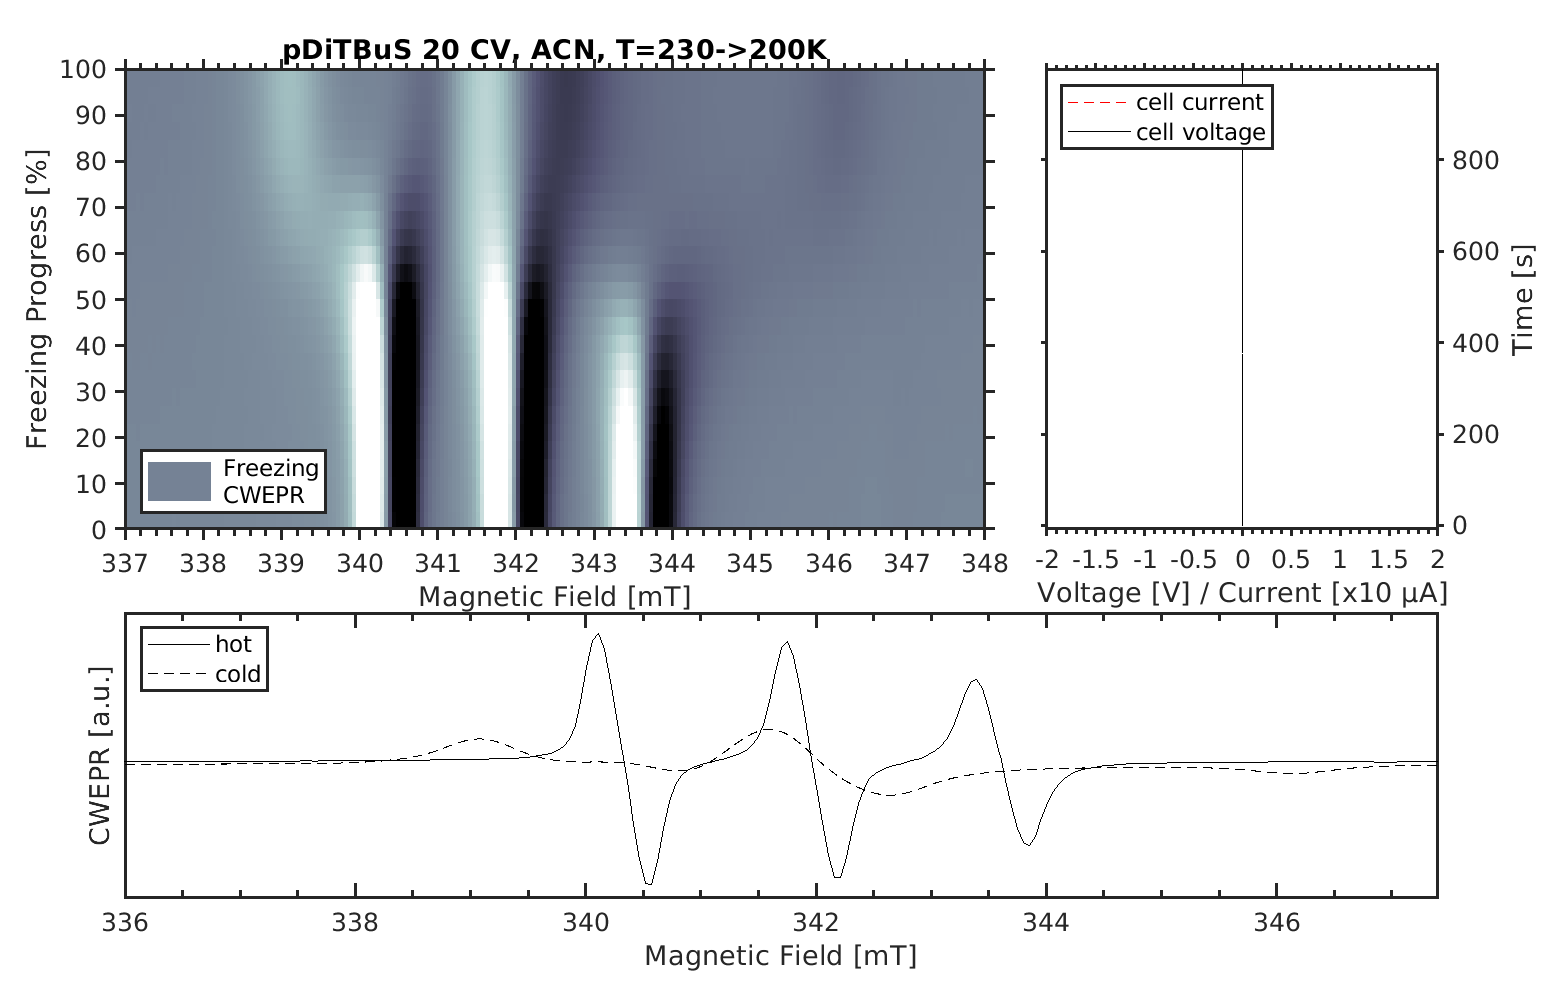
\includegraphics[width=1\textwidth]{./operando_epr/figures/CRYO/SANDWICH_FREEZING.pdf}
	\caption{Freezing a pDiTBuS cell}
	\label{fig:operando_cold_battery}
\end{figure}


\begin{figure}[h]
\center
	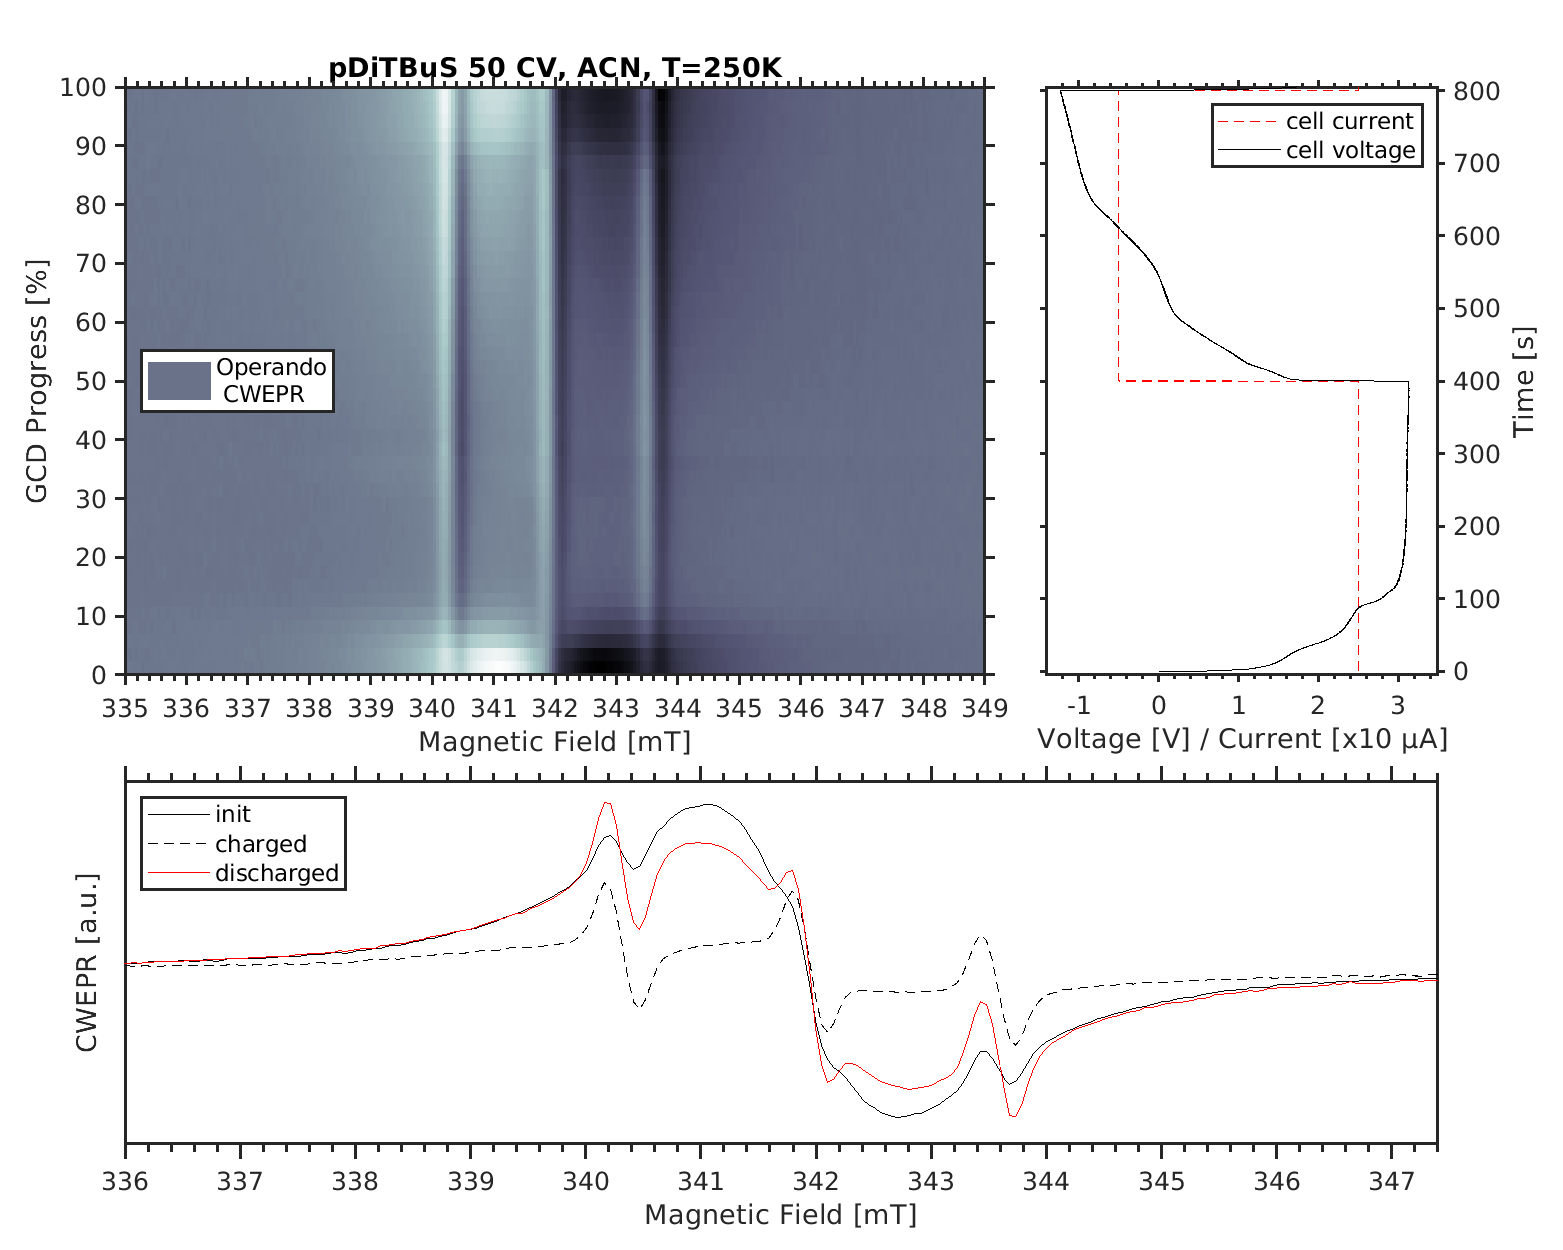
\includegraphics[width=1\textwidth]{./operando_epr/figures/slowcharge_231117_liquid_250K.pdf}
	\caption{Operando cwEPR during a charge-discharge cycle of a 2-electrode pDiTBuS electrochemical half-cell with a separator. The re-appearance of the broad spectral component indicates the reversible oxidation of the densely packed domains in the film. The three narrow lines correspond to the electrochemically inactive radicals released to the separator. Temperature decreased to 250~K to achieve a larger signal.}
	\label{fig:operando_cold_cycle}
\end{figure}


\section{EPR-Detected State Of Charge}
\label{sec:ESOC}

The SoC of the film determined with Coulomb counting were compared to quantitative cwEPR to directly relate the \ik{number of charges, injected into the film upon charging}\rs{,} to the number of paramagnetic centres in it. We refer to the \ik{fraction} of spins removed from the \ik{fully discharged} film \ik{to reach} a given SoC as the EPR-detected state of charge, or ESOC. The fully discharged film has the maximum number of spins and its ESOC is 0\%. ESOC at other SoC are determined as the fraction of the missing spins with respect to ESOC 0\%. ESOC of 95\% \rs{thus} corresponds to the oxidation state where only 5\% of the \ik{initially present} spins are left in the film. The cwEPR spectra were recorded for the listed SoC\rs{,} and the corresponding numbers of spins were calculated from the double integrals of the spectra. The integrated spectra and the experimental details are shown in the ESI, Section~\ref{si:ESOC}. \ik{The injected charges, detected spins and} ESOC values are counted for each SoC in Table~\ref{tab:Table1}. The average spin concentration in the film \rs{$\langle n\rangle$} at each ESOC was calculated from the corresponding number of spins and the estimated volume of the film of $\left(1.3\pm0.6\right)\times10^{-5}$cm$^{3}$.


\begin{table*}[!ht]

	\begin{adjustbox}{max width=\textwidth}
	 
    \begin{tblr}{ |r|c|c|c|c|c|c|c|c|}
        \toprule
E [mV] & 
SoC & 
ESOC &
capacity drawn [$\muup$Ah]& 
\ik{charges injected}&
spins \ik{detected}&
$n_{C}$~[cm$^{-3}$]&
$\langle n \rangle$~[cm$^{-3}$]&
$C$~[cm$^{-3}$] \\
		
\midrule

$ 590 \pm 5$&
$98\%$&
$(95\pm1)\%$&
\ik{$0.020\pm0.005$}&
\q{$(5\pm1)\times10^{14}$}&
\q{$(4\pm1)\times10^{14}$}&
\q{$(3\pm2)\times10^{19}$}&
\q{$(3\pm2)\times10^{19}$}&
\q{$>1\times10^{19}$}\\

\addlinespace[-0.5ex]
    
$ 500 \pm 5$&
$96\%$&
$(85\pm2)\%$&
\ik{$0.060\pm0.005$}&
\ik{$(1.4\pm0.1)\times10^{15}$}&
$(1.1\pm0.1)\times10^{15}$&
\ik{$(1.0\pm0.5)\times10^{20}$}&
\q{$(8\pm4)\times10^{19}$}&
\q{$>3\times10^{19}$}\\

\addlinespace[-0.5ex]

$ 430 \pm 5$&
$65\%$&
$(49\pm3)\%$& 
\ik{$0.480\pm0.005$}&
\ik{$(1.07\pm0.01)\times10^{16}$}&
$(3.5\pm0.2)\times10^{15}$&
\q{$(8\pm4)\times10^{20}$}&
\q{$(3\pm2)\times10^{20}$}&
$-$\\

\addlinespace[-0.5ex]

$ -200\pm 5$&
$0\%$&
$(0\pm5)\%$& 
\ik{$1.360\pm0.005$}&
\ik{$(3.05\pm0.01)\times10^{16}$}&
$(6.9\pm0.4)\times10^{15}$&
\q{$(2\pm1)\times10^{21}$}& %0.0346    0.1037    0.8297    2.3509
\q{$(5\pm3)\times10^{20}$}&
$-$\\    

        \bottomrule
    \end{tblr}
	\end{adjustbox}
	
	
\caption{EPR-detected state of charge, \ik{Coulomb counting} and the corresponding spin concentrations in a \ik{galvanostatically discharging} pDiTBuS film \ik{with $I=-10~\muup A$}. The electric potential of the film $E$ was measured with respect to the Ag/AgNO$_3$ RE. \ik{The number of injected (negative) elementary charges \rs{and the corresponding concentration of charges $n_C$ were} determined from the drawn capacity}. The average spin concentration $\langle n \rangle$ is the ratio between the number of spins measured with quantitative cwEPR and the volume of the film determined by integrating the cyclic voltammogram. $C$ is the local spin concentration in the film \ik{estimated} with \q{p}EPR as described in text.}
	
	\label{tab:Table1}	
	
	
\end{table*}

\subsection{Formation of Singlet Spin States in a Discharged Cathode}
The number of electrons left in the film were determined with the Coulomb counting from the galvanostatic discharge curves shown in Figure~\ref{fig:Figure_S27}. The number of electron spins detected with cwEPR is close to the Coulomb counting for high SoC, that corresponds to lower spin concentrations. However, for low SoC, the difference in the number of electrons measured with the Coulomb counting and with quantitative cwEPR is dramatic: up to 70\% of the electrons in the discharged film are EPR silent. The absence of cwEPR signal from the majority of the electrons indicates that their spins pair up in singlet (S=0) EPR silent states. The singlet spin pairs follow Bose statistics and can occupy the same quantum state which is favorable for the charge transport. The formation of singlet states was detected only in low SoC.











